%%!!!!!!!!!!!!!!!!!!!!!!!!!!!!!!!!!!!!!!!!!!!!!!!!!!!!!!!!!!!!!!!!!!!!!!!!!!!!!!
%%%%%%%%%%%%%%%%%%%%%%%%%%%%%%%%%%%%%%%%%%%%%%%%%%%%%%%%%%%%%%%%%%%%%%%%%%%%%%%%
%% SECTION: Przygotowanie eksperymentu
%%%%%%%%%%%%%%%%%%%%%%%%%%%%%%%%%%%%%%%%%%%%%%%%%%%%%%%%%%%%%%%%%%%%%%%%%%%%%%%%
%%!!!!!!!!!!!!!!!!!!!!!!!!!!!!!!!!!!!!!!!!!!!!!!!!!!!!!!!!!!!!!!!!!!!!!!!!!!!!!!
\section{Przygotowanie eksperymentu}

Eksperymentalna część pracy bezsprzecznie wymaga przygotowania odpowiedniego zestawu
sprzętu i~narzędzi. Konieczne jest wybranie odpowiedniej platformy sprzętowej
wspierającej komunikację bezprzewodową Bluetooth Low Energy w wersji minimum 5.0.
Niezbędne jest również oprzyrządowanie pomiarowe, które umożliwia pomiar natężeń
prądu poniżej 1mA, ze względu na energooszczędność urządzeń \gls{BLE}.

% zakładam, że we wcześniejszych rozdziałach definiuję zakres pracy i rodzaje eksperymentów

Badania zużycia energii wymagają aparatury, która w pełni zarejestruje minima i maksima
poboru prądu przy niskich błędach pomiarowych.

Eksperyment \gls{PER} wymaga przygotowania wielu zestawów uruchomieniowych obsługujących
komunikację BLE w konfiguracji Mesh. Dodatkowo, wymagane jest stworzenie dedykowanego oprogramowania
na mikrokontroler jak i komputer osobisty. Jest to niezbędne w celu kontroli przepływu
doświadczenia jak i akwizycji danych.

Niniejszy rozdział omawia zakres przygotowań do przeprowadzenia właściwych eksperymentów.


%%%%%%%%%%%%%%%%%%%%%%%%%%%%%%%%%%%%%%%%%%%%%%%%%%%%%%%%%%%%%%%%%%%%%%%%%%%%%%%%
%% SUBSECTION: Sprzęt i oprzyrządowanie
%%%%%%%%%%%%%%%%%%%%%%%%%%%%%%%%%%%%%%%%%%%%%%%%%%%%%%%%%%%%%%%%%%%%%%%%%%%%%%%%
\subsection{Sprzęt i oprzyrządowanie}

Próby doświadczalne oparto o produkty firmy ST. Decyzja podjęta została w oparciu
o osobiste preferencje autora pracy.

\subsubsection{P-NUCLEO-WB55}

Badania Bluetooth Low Energy wymagały wyboru platformy, która umożliwia eksperymentalną 
weryfikację wybranych celów badawczych. Ostatecznie, zdecydowano się na wykorzystanie 
mikrokontrolera \textit{STM32WB55RG}. W celu zapewnienia powtarzalności eksperymentu jak 
i~ze względu na ograniczenia czasowe, docelową platformą badawczą stał się zestaw 
uruchomieniowy \textit{P-NUCLEO-WB55}~\cite{noauthor_p-nucleo-wb55_nodate}.

Zestaw ten zgodny jest ze specyfikacją Bluetooth Low Energy v5.0. Dodatkowo, wspiera
on inne standardy komunikacji, m.in. Zigbee \cite{noauthor_stm32wb_2022}.
Ten fakt może zostać wykorzystany w celu bezpośredniego porównania różnych stosów komunikacji bezprzewodowej.
Nie jest to jednak celem niniejszej pracy, a stanowi możliwość jej dalszego 
rozwinięcia.


\begin{figure}[!htb]
	\centering 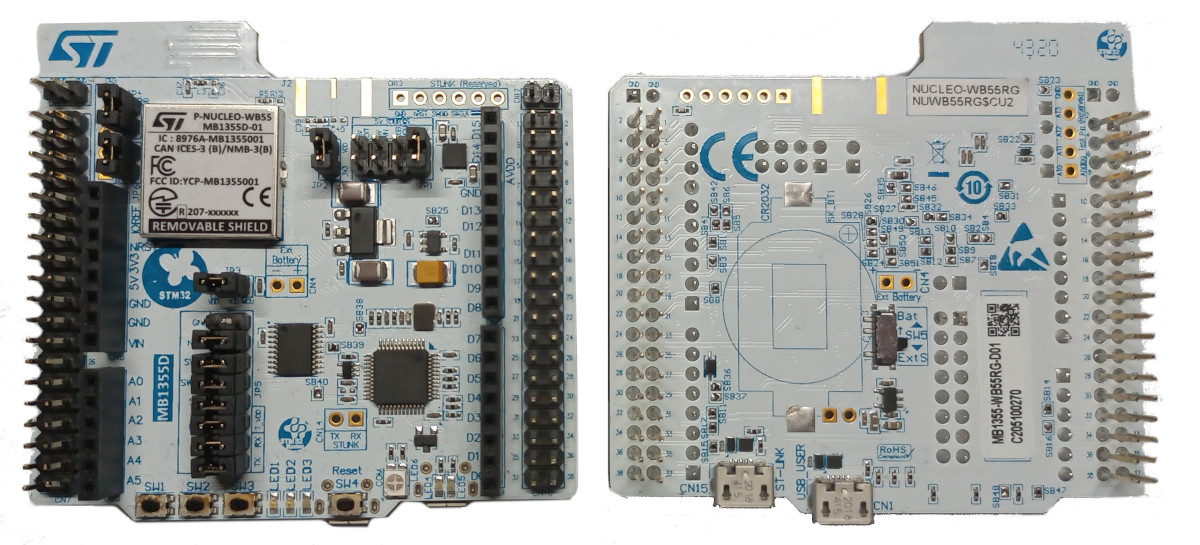
\includegraphics[width=0.618\linewidth]{nucleo_wb55.jpg}
	\caption{Zestaw uruchomieniowy P-NUCLEO-WB55. Źródło: \cite{noauthor_p-nucleo-wb55_nodate}}
	\label{rys:nucleo_wb55}
\end{figure}

\subsubsection{X-NUCLEO-LPM01A}

Płytka rozszerzeń X-NUCLEO-LPM01A spełnia wszelkie oczekiwania dotyczące możliwości pomiarowych
stawianych przed projektem. Wg oficjalnej dokumentacji \cite{noauthor_um2243_2018}, układ oferuje:

\begin{itemize}
\item Programowalne źródło napięciowe 1,8V do 3,3V
\item Dynamiczne próbkowanie w zakresie od 100nA 50mA przy maksymalnej częstotliwości 100kHz z 2\%-ową dokładnością pomiarów
\item Pomiar statyczny natężenia prądu do 200mA
\item Integracja z aplikacją do dedykowaną aplikacją akwizycji danych \cite{noauthor_stm32cubemonpwr_2022}
\end{itemize}

\begin{figure}[!ht]
	\centering 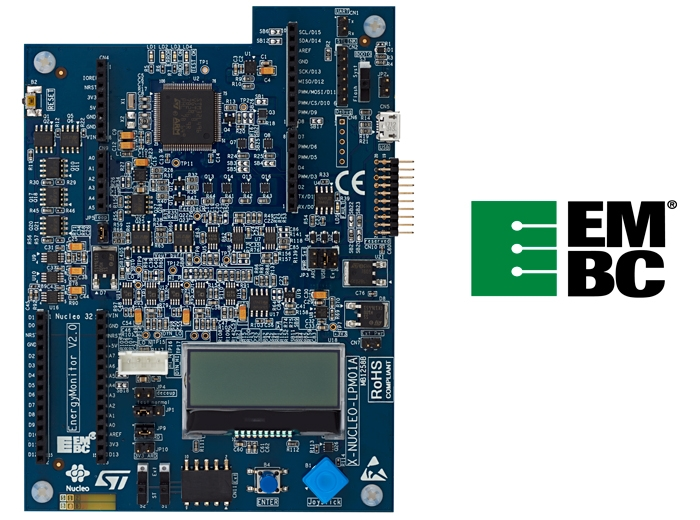
\includegraphics[width=0.618\linewidth]{st_power_measurement_unit.jpg}
	\caption{Zestaw pomiarowy X-NUCLEO-LPM01A. Źródło: \cite{noauthor_x-nucleo-lpm01a_nodate}}
	\label{rys:nucleo_lpm01a}
\end{figure}

Moduł ten nie ogranicza się tylko do wykorzystywania autorskich złącz firmy ST. Schemat wyprowadzeń pinów
umożliwia wykorzystanie popularnych platform takich jak Arduino\footnote{https://www.arduino.cc/}. Co istotniejsze, wybrana płytka umożliwia
zasilanie dowolnego układu dzięki wyprowadzeniu źródła napięciowego za pośrednictwem pinów 
(za dokumentacją: złącze CN14). Ten fakt został wykorzystany w badaniach, pozwalając uniknąć kłopotliwej
konfiguracji P-NUCLEO-WB55 wymagającej tworzenia dodatkowych ścieżek lutowanych.

Dodatkową cechą tego modułu jest akwizycja danych z użyciem komputera osobistego. Dzięki dedykowanej
aplikacji, dostarczanej wraz z modułem, możliwa jest akwizycja danych w czasie rzeczywistym przy
wybranych częstotliwościach próbkowania. Zebrane w ten sposób dane służą dalszym analizom, co zostało
wykorzystane w niniejszej pracy. 

\subsubsection{Narzędzia i firmware firmy ST}
Firma ST wraz z zestawem uruchomieniowym udostępnia pełne zintegrowane środowisko
programistyczne oraz niezbędne biblioteki i certyfikowany firmware:

\begin{itemize}
\item \textbf{STM32CubeIDE} \cite{noauthor_stm32cubeide_2022} - multiplatformowe zintegrowane środowisko programistyczne
dostarczane przez ST bazujące na otwartoźródłowym środowisko \textit{Eclipse}\footnote{https://www.eclipse.org/ide/}.
\item \textbf{STM32CubeProgrammer} \cite{noauthor_stm32cubeprog_2022} - narzędzie umożliwiające wykonywanie operacji
odczytu, zapisu i weryfikacji skompilowanego oprogramowania produktów STM32. 
\item \textbf{STM32CubeMonitor-Power} \cite{noauthor_stm32cubemonpwr_2022} - oprogramowanie służące akwizycji danych
o zużyciu energii m.in. w zestawie X-NUCLEO-LPM01A Rysunek: \ref{rys:nucleo_lpm01a}.
\item \textbf{Firmware STM32CubeWB} \cite{noauthor_stm32cubewb_2022} - zestaw bibliotek, narzędzi oraz przykładów
przeznaczonych dla mikrokontrolerów rodziny STM32WB. W skład tego repozytorium wchodzą zależności takie jak:
skompilowany, zamknięty firmware ko-processora dla różnych stosów połączeń bezprzewodowych; przykłady programów
wykorzystujące biblioteki HAL jak i również bezpośrednio rejestry; przykłady BLE; przykłady BLE Mesh.
\end{itemize}

%%%%%%%%%%%%%%%%%%%%%%%%%%%%%%%%%%%%%%%%%%%%%%%%%%%%%%%%%%%%%%%%%%%%%%%%%%%%%%%%
%% SUBSECTION: Zasilanie i obudowy
%%%%%%%%%%%%%%%%%%%%%%%%%%%%%%%%%%%%%%%%%%%%%%%%%%%%%%%%%%%%%%%%%%%%%%%%%%%%%%%%
\subsection{Narzędzia i elementy dodatkowe}

\subsubsection{Zasilanie}
Próby terenowe wymagają odrębnego, właściwego zasilania. Wybrane zestawy uruchomieniowe
wykorzystują ustandaryzowane złącze komunikacyjne USB. Złącze to oprócz komunikacji
oferuje zasilanie linią +5V. Przeprowadzając właściwe eksperymenty wykorzystano
komercyjnie dostępne banki energii tzw. powerbanki. Są to akumulatory litowo-jonowe
lub litowo-polimerowe z wbudowanym systemem zarządzania baterią\footnote{\gls{BMS} - ang. Battery Management System}
i właściwymi przetwornicami impulsowymi w celu zapewnienia odpowiedniego napięcia zasilania.

Elektronika wbudowane w magazyny energii automatycznie wyłącza zasilanie w przypadku braku
podłączonego urządzenia lub gdy dane urządzenie pobiera marginalnie niskie wartości
prądu. Służy to ochronie cennego i delikatnego akumulatora. Jest to cecha korzystna
z punktu widzenia konsumenta kupującego powerbank w celu szybkiego ładowania urządzeń elektronicznych.
Niestety, zaleta ta staje się wadą w przypadku przeprowadzanych doświadczeń. Podłączając moduł P-NUCLEO-WB55,
urządzenie po pewnym okresie działania wyłącza się na skutek uruchomionych zabezpieczeń w źródle energii.

W celu skonstruowano trywialne urządzenie, które wlutowane równolegle w linię zasilania 5V,
konsumuje ok. 100mA prądu (0,5W = 5V * 0,02A * 5 [diod]). Doświadczalnie stwierdzono, że tak włączony
odbiornik energii umożliwia stabilne działanie włączonego do sieci modułu STM32. Schemat 
zaprezentowano na Rysunku~\ref{rys:power_led_consumer}

\begin{figure}[!ht]
	\centering 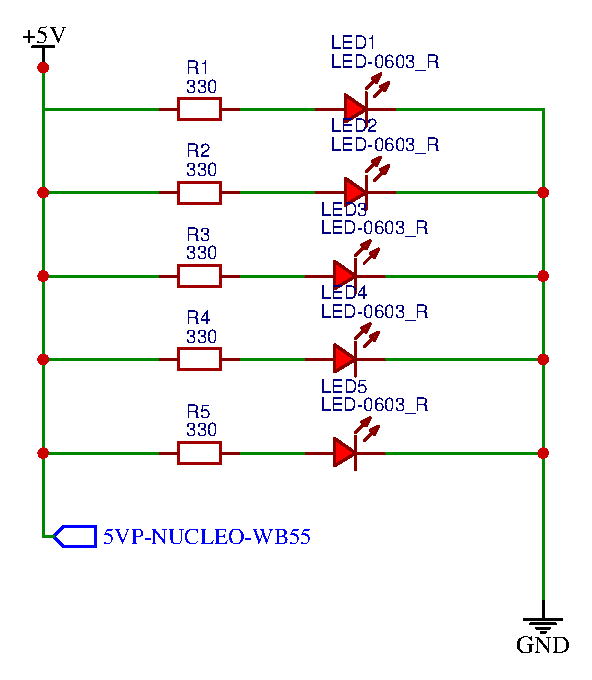
\includegraphics[width=0.618\linewidth]{power_led_consumer.pdf}
	\caption{Odbiornik energii}
	\label{rys:power_led_consumer}
\end{figure}

\subsubsection{Obudowa - druk 3D}
Kolejnym elementem niezbędnym w celu przeprowadzenia eksperymentów terenowych jest zapewnienie
ochrony mechanicznej wybranych zestawów uruchomieniowych. Podczas prób elementy mogą zostać
fizycznie uszkodzone poprzez m.in. wyłamanie fragmentu \gls{PCB} (w tym anteny), uszkodzenie pinów etc.

Wykorzystując techniki projektowania wspomaganego komputerowo\footnote{\gls{CAD} - ang. \textit{Computer-aided Design}},
zaprojektowano autorską obudowę. Głównym celem projektowym było zapewnienie minimalnej ochrony
mechanicznej, jednocześnie redukując możliwy wpływ materiału na tłumienie sygnału. Elementy
interfejsu: przyciski i~antena, zostały celowo wyeksponowane. Rzut izometryczny przedstawiony został
na Rysunku~\ref{rys:obudowa_model3d}.


\begin{figure}[!htb]
	\centering 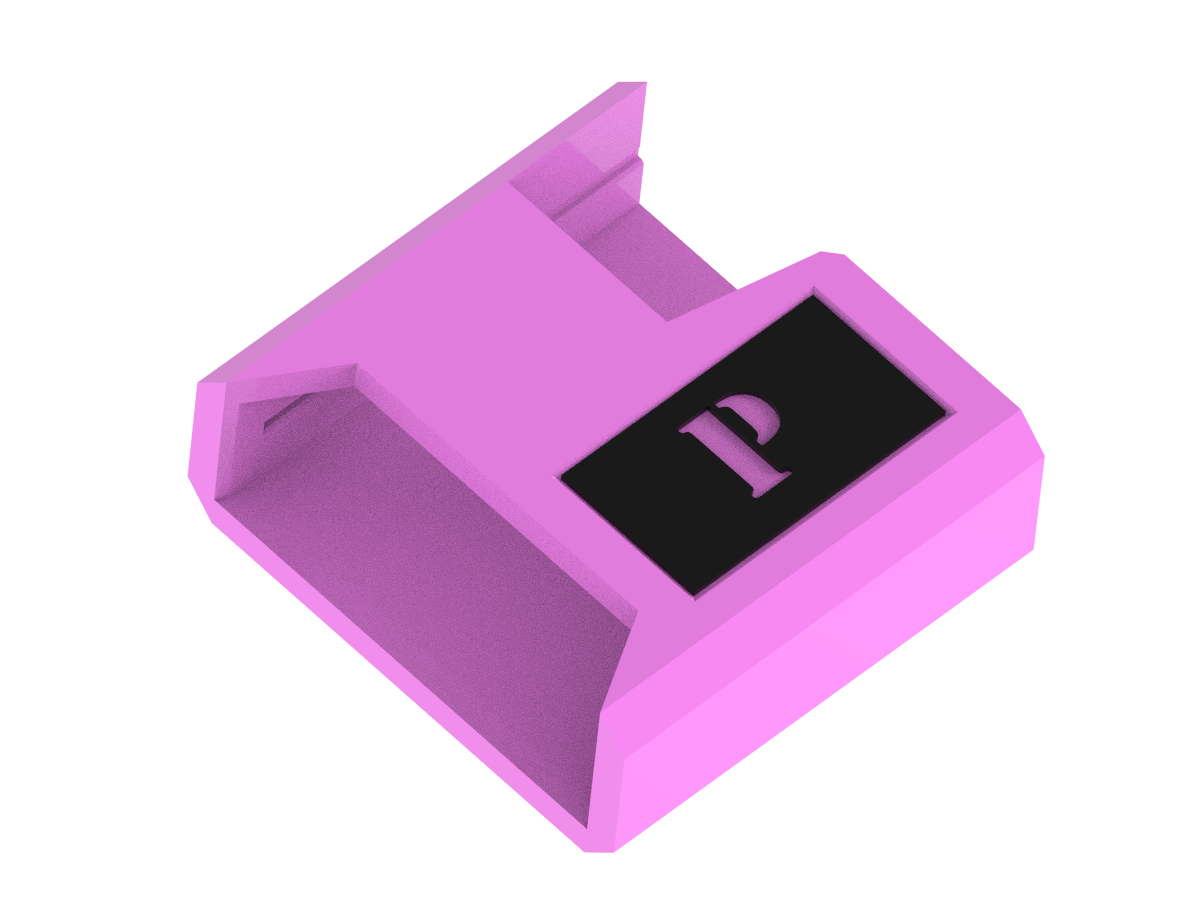
\includegraphics[width=0.618\linewidth]{stm_case_render.png}
	\caption{Model obudowy dla zestawu P-NUCLEO-WB55}
	\label{rys:obudowa_model3d}
\end{figure}

Obudowa wykonana została z materiału \gls{PLA}\footnote{PLA - ang. \textit{Polylactic acid}, polilaktyd} techniką
druku 3D \gls{FDM}\footnote{FDM - ang. \textit{Fused Deposition Modeling}}/\gls{FFF}\footnote{FFF - \textit{Fused Filament Fabrication}}.
Jednobryłowa konstrukcja podyktowana została chęcią uproszczenia wydruku, kosztem zwiększonych trudności
doboru tolerancji dla umieszczanych wewnątrz płytek \gls{PCB}. Obudowa przewiduje wsuwanie modułu Nucleo
do wewnątrz, zapewniając jednoczesne pewne jego mocowanie.

Dobór koloru wydruku również nie był przypadkowy. Przewidując potencjalne lokalizacje przeprowadzanych
doświadczeń, wybrano kolor możliwie jaskrawy. Podstawowym założeniem było ułatwienie dostrzeżenia
obudowy, a wraz z obudową również zestawu uruchomieniowego, pośród flory leśnej czy terenów
zurbanizowanych. Ostateczne wykonanie obudów zaprezentowano na Rysunku~\ref{rys:obudowa_wykonanie}.

\begin{figure}[!htb]
	\centering 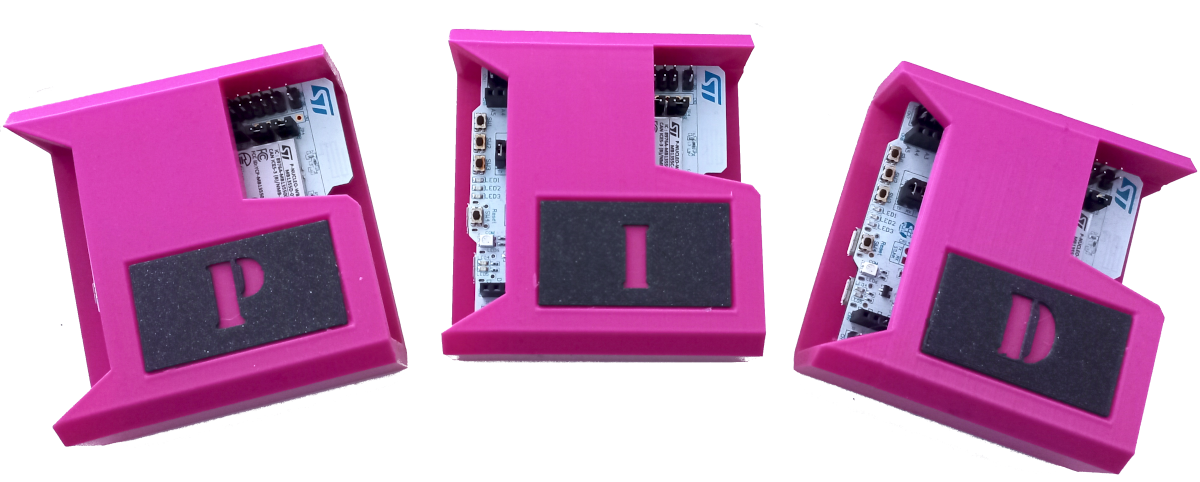
\includegraphics[width=0.618\linewidth]{3d_real_cases.png}
	\caption{Obudowa zestawu uruchomieniowego Nucleo wykonana w technologii druku 3D - realizacja}
	\label{rys:obudowa_wykonanie}
\end{figure}

%%%%%%%%%%%%%%%%%%%%%%%%%%%%%%%%%%%%%%%%%%%%%%%%%%%%%%%%%%%%%%%%%%%%%%%%%%%%%%%%
%% SUBSECTION: Oprogramowanie mikrokontrolera
%%%%%%%%%%%%%%%%%%%%%%%%%%%%%%%%%%%%%%%%%%%%%%%%%%%%%%%%%%%%%%%%%%%%%%%%%%%%%%%%
\subsection{Oprogramowanie mikrokontrolera} \label{prep:uc-software}

\begin{lstlisting}[language=C,
    caption={Testowy kod C},
    label={lst:kod cpp}]
MOBLE_RESULT Appli_Generic_OnOff_Set(Generic_OnOffStatus_t* pGeneric_OnOffParam, 
                                     MOBLEUINT8 OptionalValid,
                                     MOBLEUINT16 dstPeer,
                                     MOBLEUINT8 elementIndex)
{
  /* LED control only for main element */
  if(elementIndex == GENERIC_SERVER_MAIN_ELEMENT_INDEX)
  {
  // [...]
      if(AppliOnOffSet[elementIndex].Present_OnOffValue == AppliOnOffSet[elementIndex].TargetValue)
      {
    	if (dstPeer != 0xc000) {
    	   increment_generic_onoff_counter_packet_error_rate_experiment(AppliOnOffSet[elementIndex].Present_OnOffValue, dstPeer);
    	}
        if(AppliOnOffSet[elementIndex].Present_OnOffValue > 0)
        {
          BSP_LED_On(LED_BLUE);
        }
        else
        {
          BSP_LED_Off(LED_BLUE);
        }
      }
    }  
  // [...]
\end{lstlisting}

%%%%%%%%%%%%%%%%%%%%%%%%%%%%%%%%%%%%%%%%%%%%%%%%%%%%%%%%%%%%%%%%%%%%%%%%%%%%%%%%
%% SUBSECTION: Oprogramowanie PC
%%%%%%%%%%%%%%%%%%%%%%%%%%%%%%%%%%%%%%%%%%%%%%%%%%%%%%%%%%%%%%%%%%%%%%%%%%%%%%%%
\subsection{Oprogramowanie PC}


%%!!!!!!!!!!!!!!!!!!!!!!!!!!!!!!!!!!!!!!!!!!!!!!!!!!!!!!!!!!!!!!!!!!!!!!!!!!!!!!
%%%%%%%%%%%%%%%%%%%%%%%%%%%%%%%%%%%%%%%%%%%%%%%%%%%%%%%%%%%%%%%%%%%%%%%%%%%%%%%%
%% SECTION: Zużycie energii
%%%%%%%%%%%%%%%%%%%%%%%%%%%%%%%%%%%%%%%%%%%%%%%%%%%%%%%%%%%%%%%%%%%%%%%%%%%%%%%%
%%!!!!!!!!!!!!!!!!!!!!!!!!!!!!!!!!!!!!!!!!!!!!!!!!!!!!!!!!!!!!!!!!!!!!!!!!!!!!!!
\section{Zużycie energii}

%%%%%%%%%%%%%%%%%%%%%%%%%%%%%%%%%%%%%%%%%%%%%%%%%%%%%%%%%%%%%%%%%%%%%%%%%%%%%%%%
%% SUBSECTION: Metodologia badania
%%%%%%%%%%%%%%%%%%%%%%%%%%%%%%%%%%%%%%%%%%%%%%%%%%%%%%%%%%%%%%%%%%%%%%%%%%%%%%%%
\subsection{Metodologia badania}

\lipsum[1-3]
%%%%%%%%%%%%%%%%%%%%%%%%%%%%%%%%%%%%%%%%%%%%%%%%%%%%%%%%%%%%%%%%%%%%%%%%%%%%%%%%
%% SUBSECTION: BT Low Energy - Usługa Heart Rate
%%%%%%%%%%%%%%%%%%%%%%%%%%%%%%%%%%%%%%%%%%%%%%%%%%%%%%%%%%%%%%%%%%%%%%%%%%%%%%%%
\subsection{BT Low Energy - Usługa Heart Rate}

\lipsum[1-3]
\begin{figure}[!htb]
	\centering 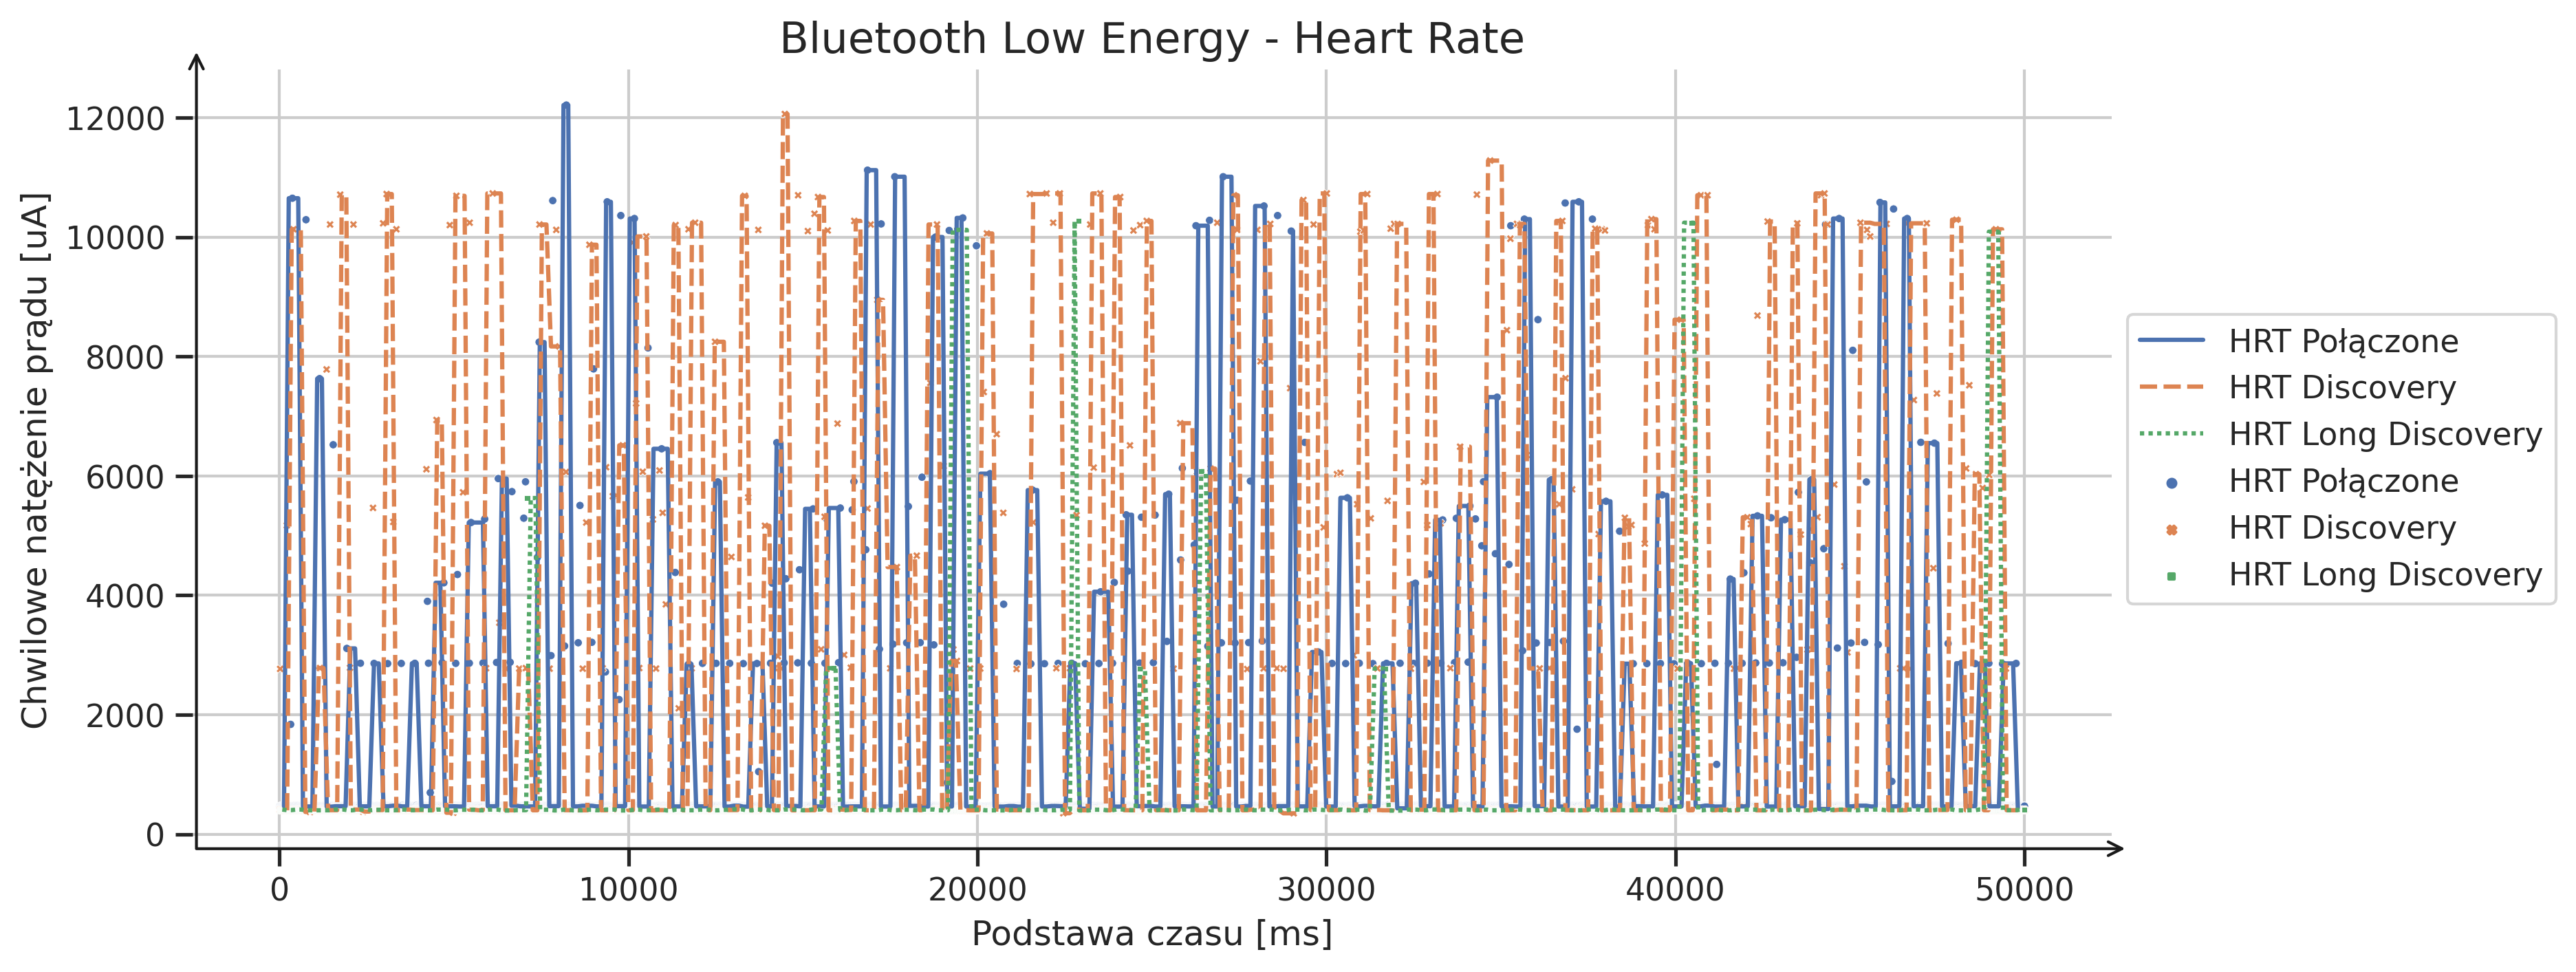
\includegraphics[width=0.99\linewidth]{power_ble_hr_amps.png}
	\caption{Charakterystyka czasowa poboru prądu dla BLE i usługi Heart Rate}
	\label{rys:power_ble_hr_amps}
\end{figure}

\lipsum[1-2]
\begin{figure}[!htb]
	\centering 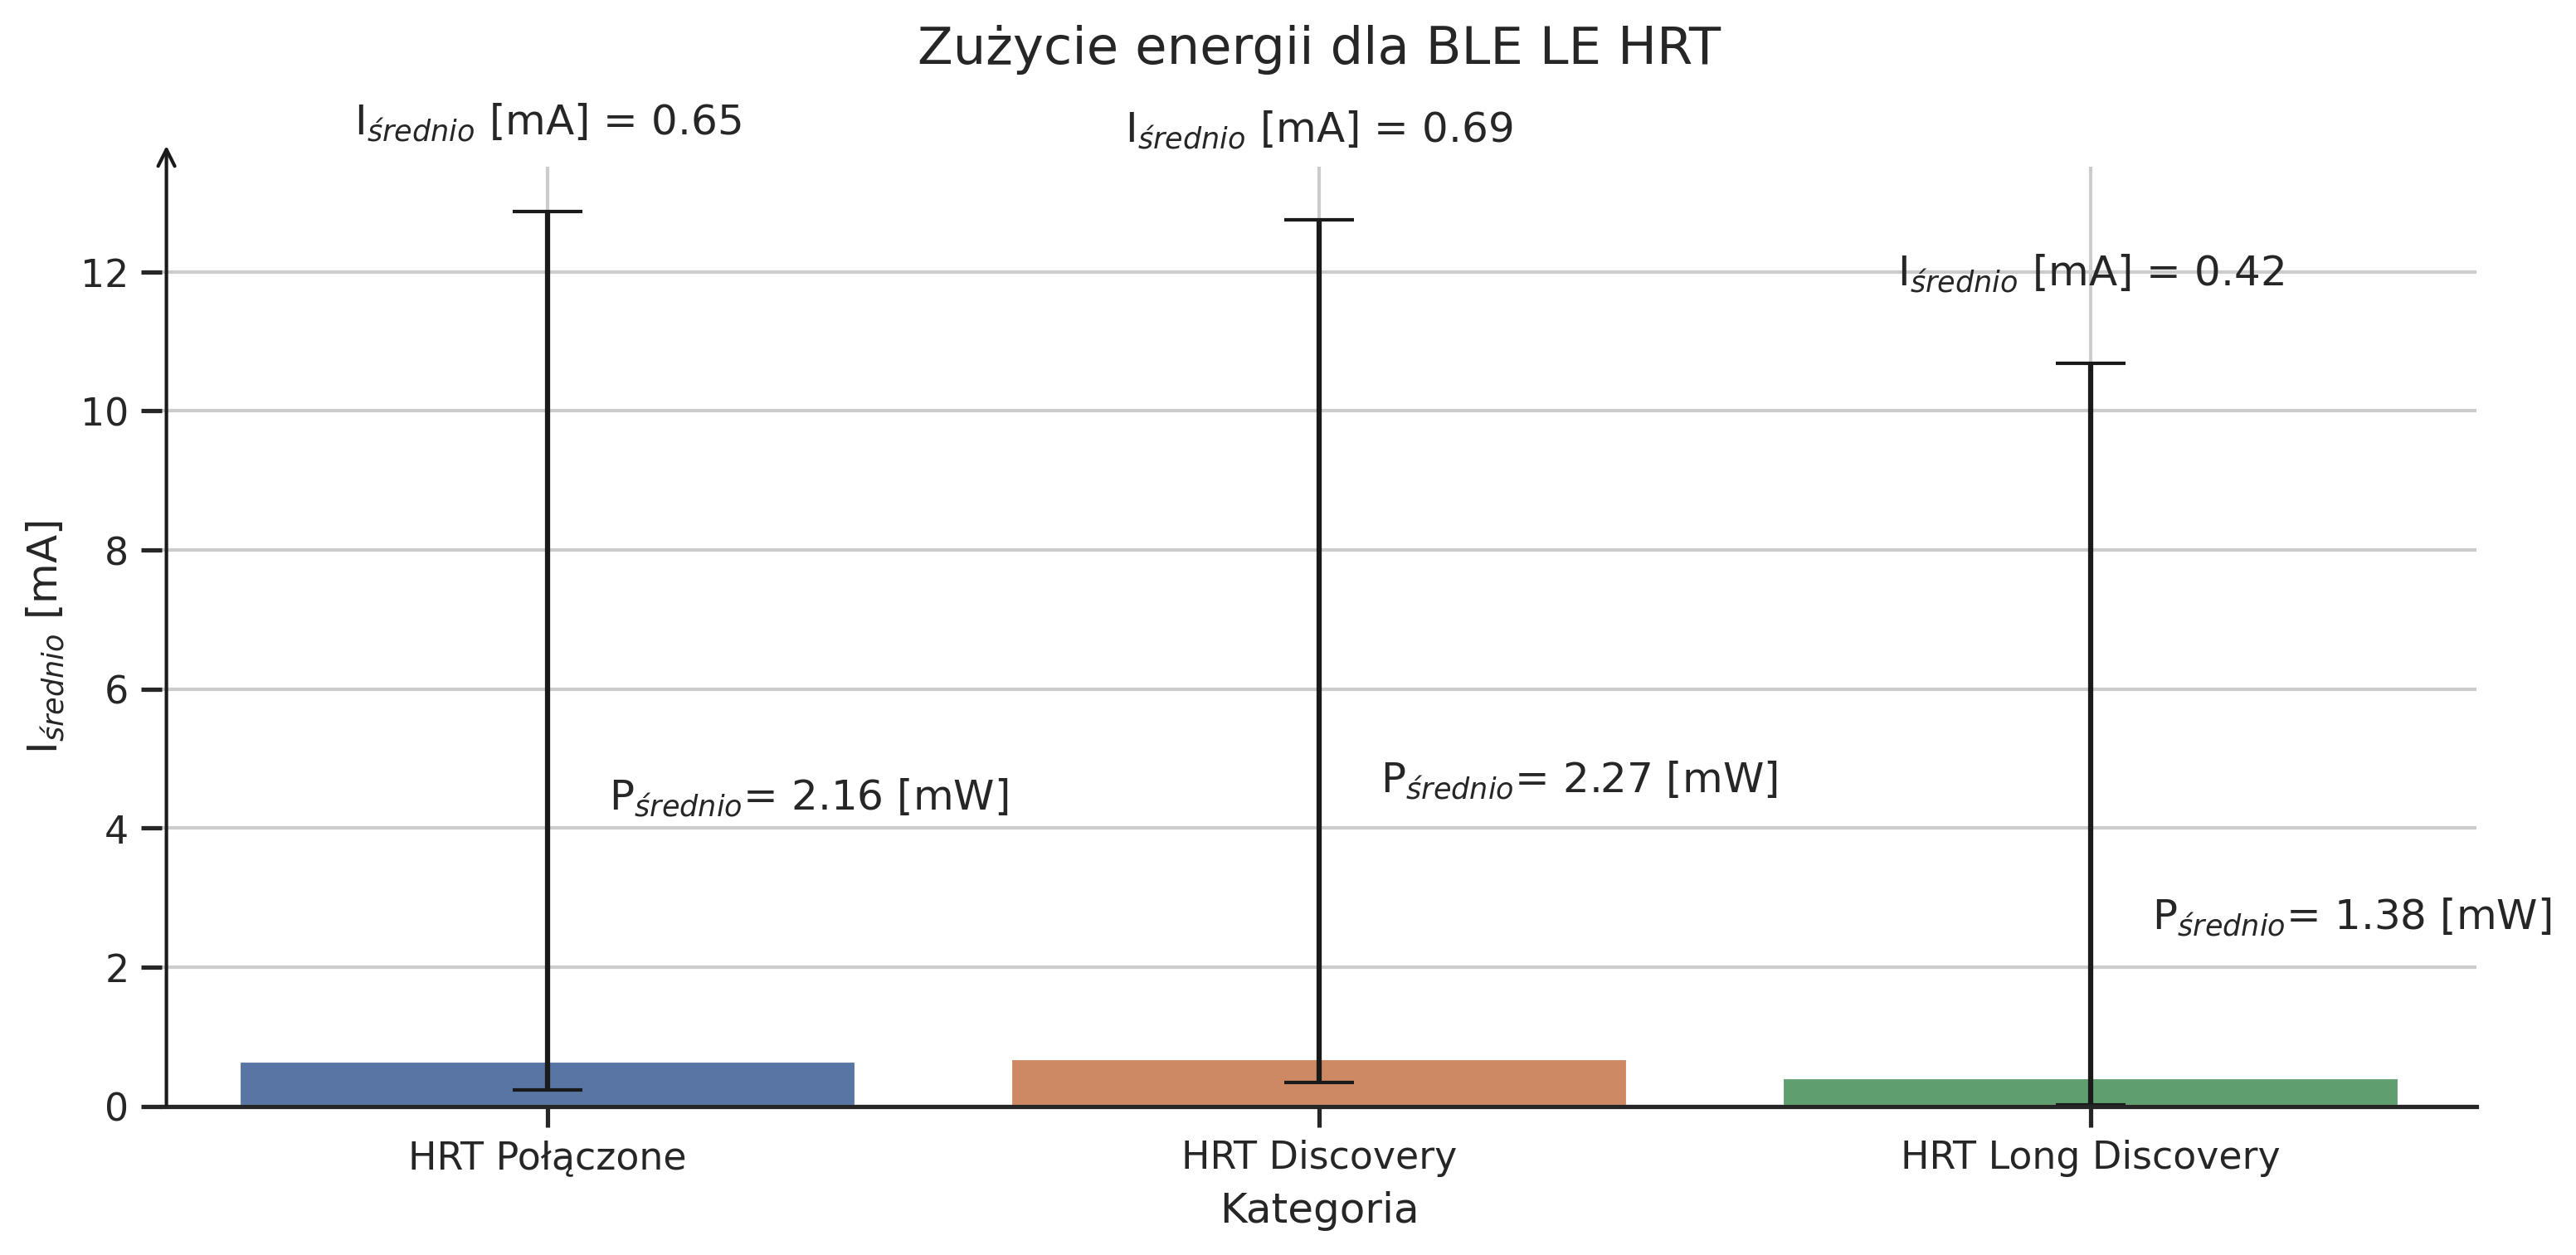
\includegraphics[width=0.99\linewidth]{power_ble_hr_amps_usage_juxtaposition.png}
	\caption{Zestawienie zużycia prądu dla usługi Heart Rate w zależności od trybu działania}
	\label{rys:power_ble_hr_amps_usage_juxtaposition}
\end{figure}
\lipsum[1-3]

%%%%%%%%%%%%%%%%%%%%%%%%%%%%%%%%%%%%%%%%%%%%%%%%%%%%%%%%%%%%%%%%%%%%%%%%%%%%%%%%
%% SUBSECTION: BLE Mesh - Model Generic OnOff
%%%%%%%%%%%%%%%%%%%%%%%%%%%%%%%%%%%%%%%%%%%%%%%%%%%%%%%%%%%%%%%%%%%%%%%%%%%%%%%%
\subsection{BLE Mesh - Model Generic OnOff}

Pomiary dla BLE Mesh uwzględniające dwa tryby działania: sieć w oczekująca na komunikaty oraz podczas działania aktywnego korzystania z Modelu Generic OnOff.

\begin{figure}[!htb]
	\centering 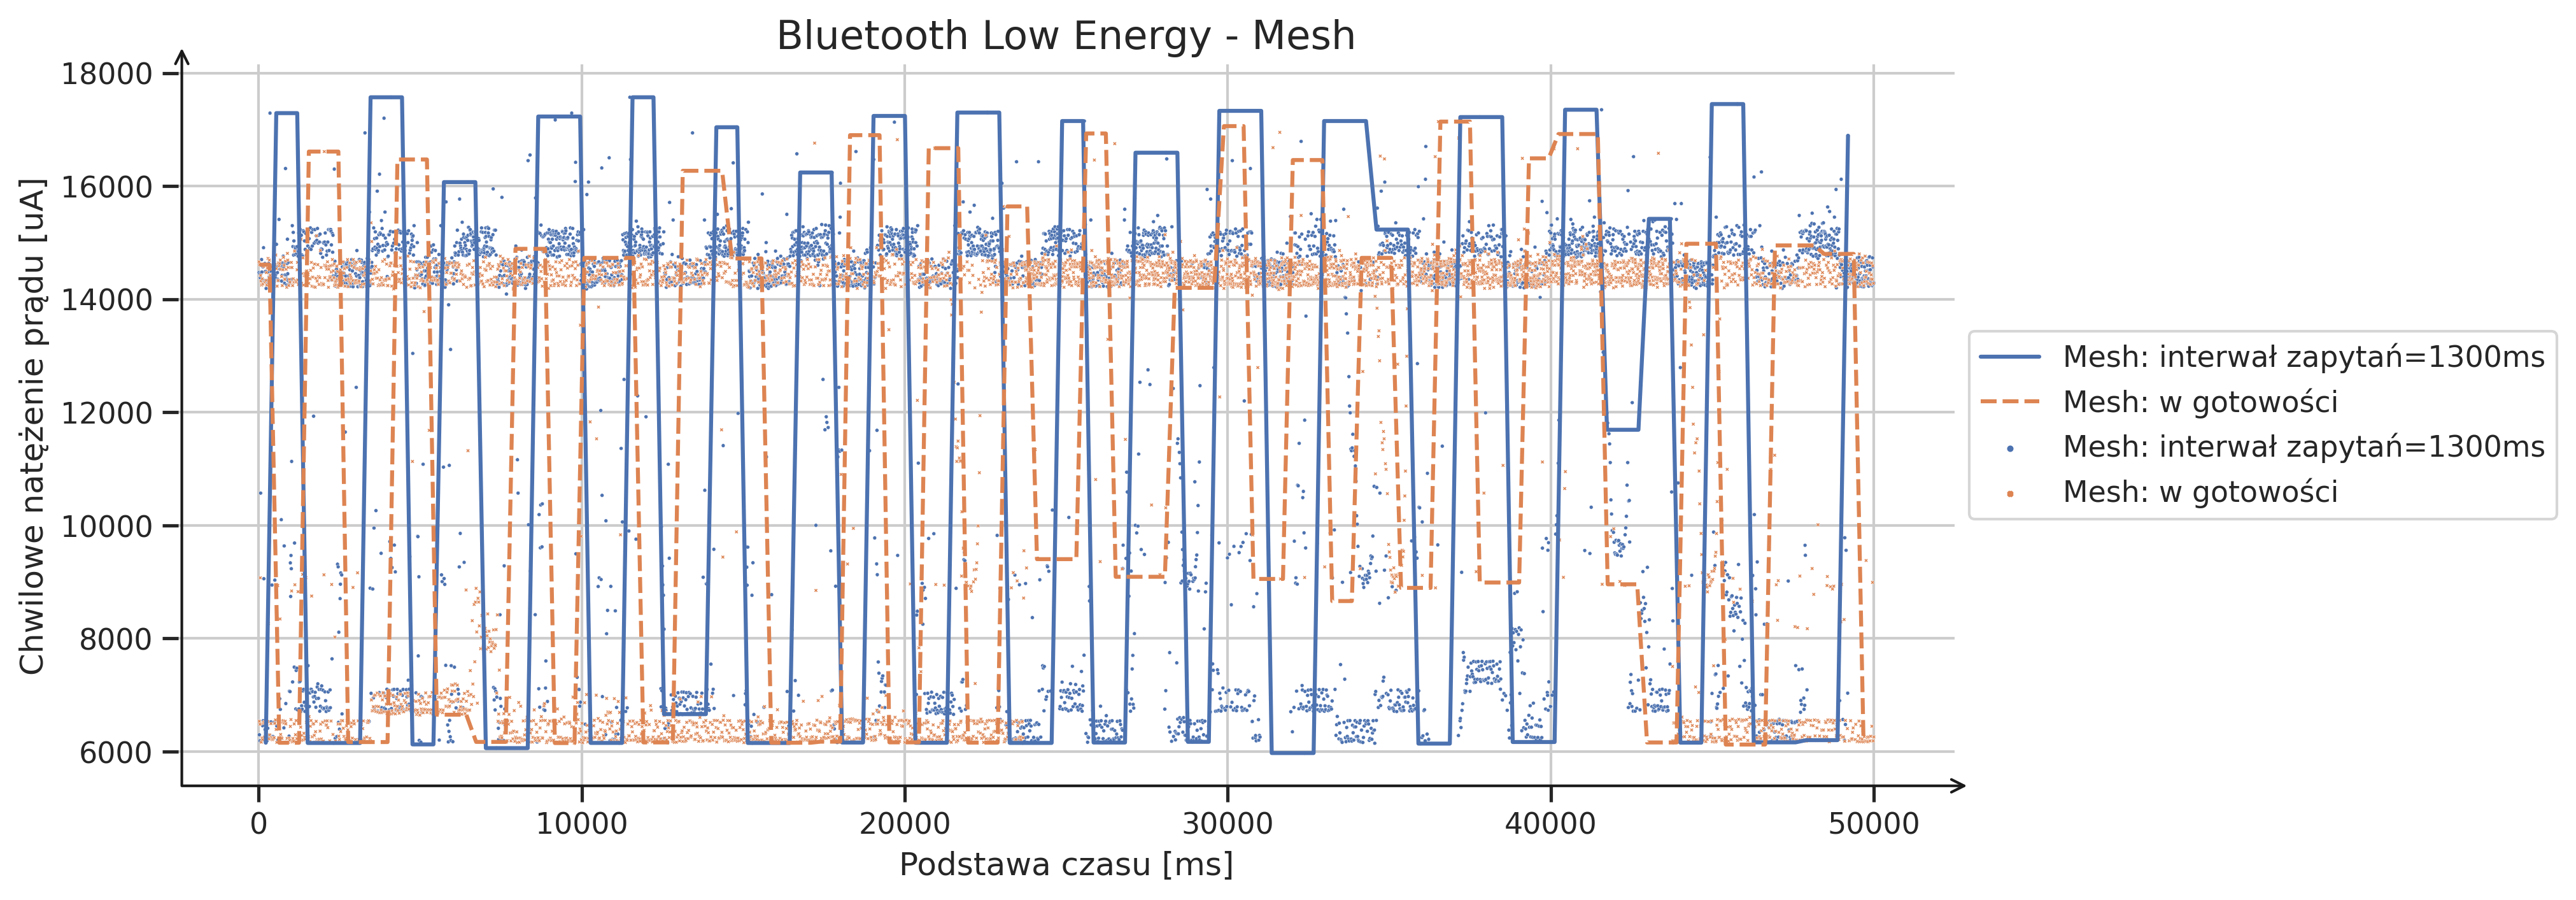
\includegraphics[width=0.99\linewidth]{power_ble_mesh_amps.png} 
	\caption{Charakterystyka czasowa poboru prądu dla BLE Mesh i modelu Generic OnOff}
	\label{rys:power_ble_mesh_amps}
\end{figure}

\lipsum[1-3]
\begin{figure}[!htb]
	\centering 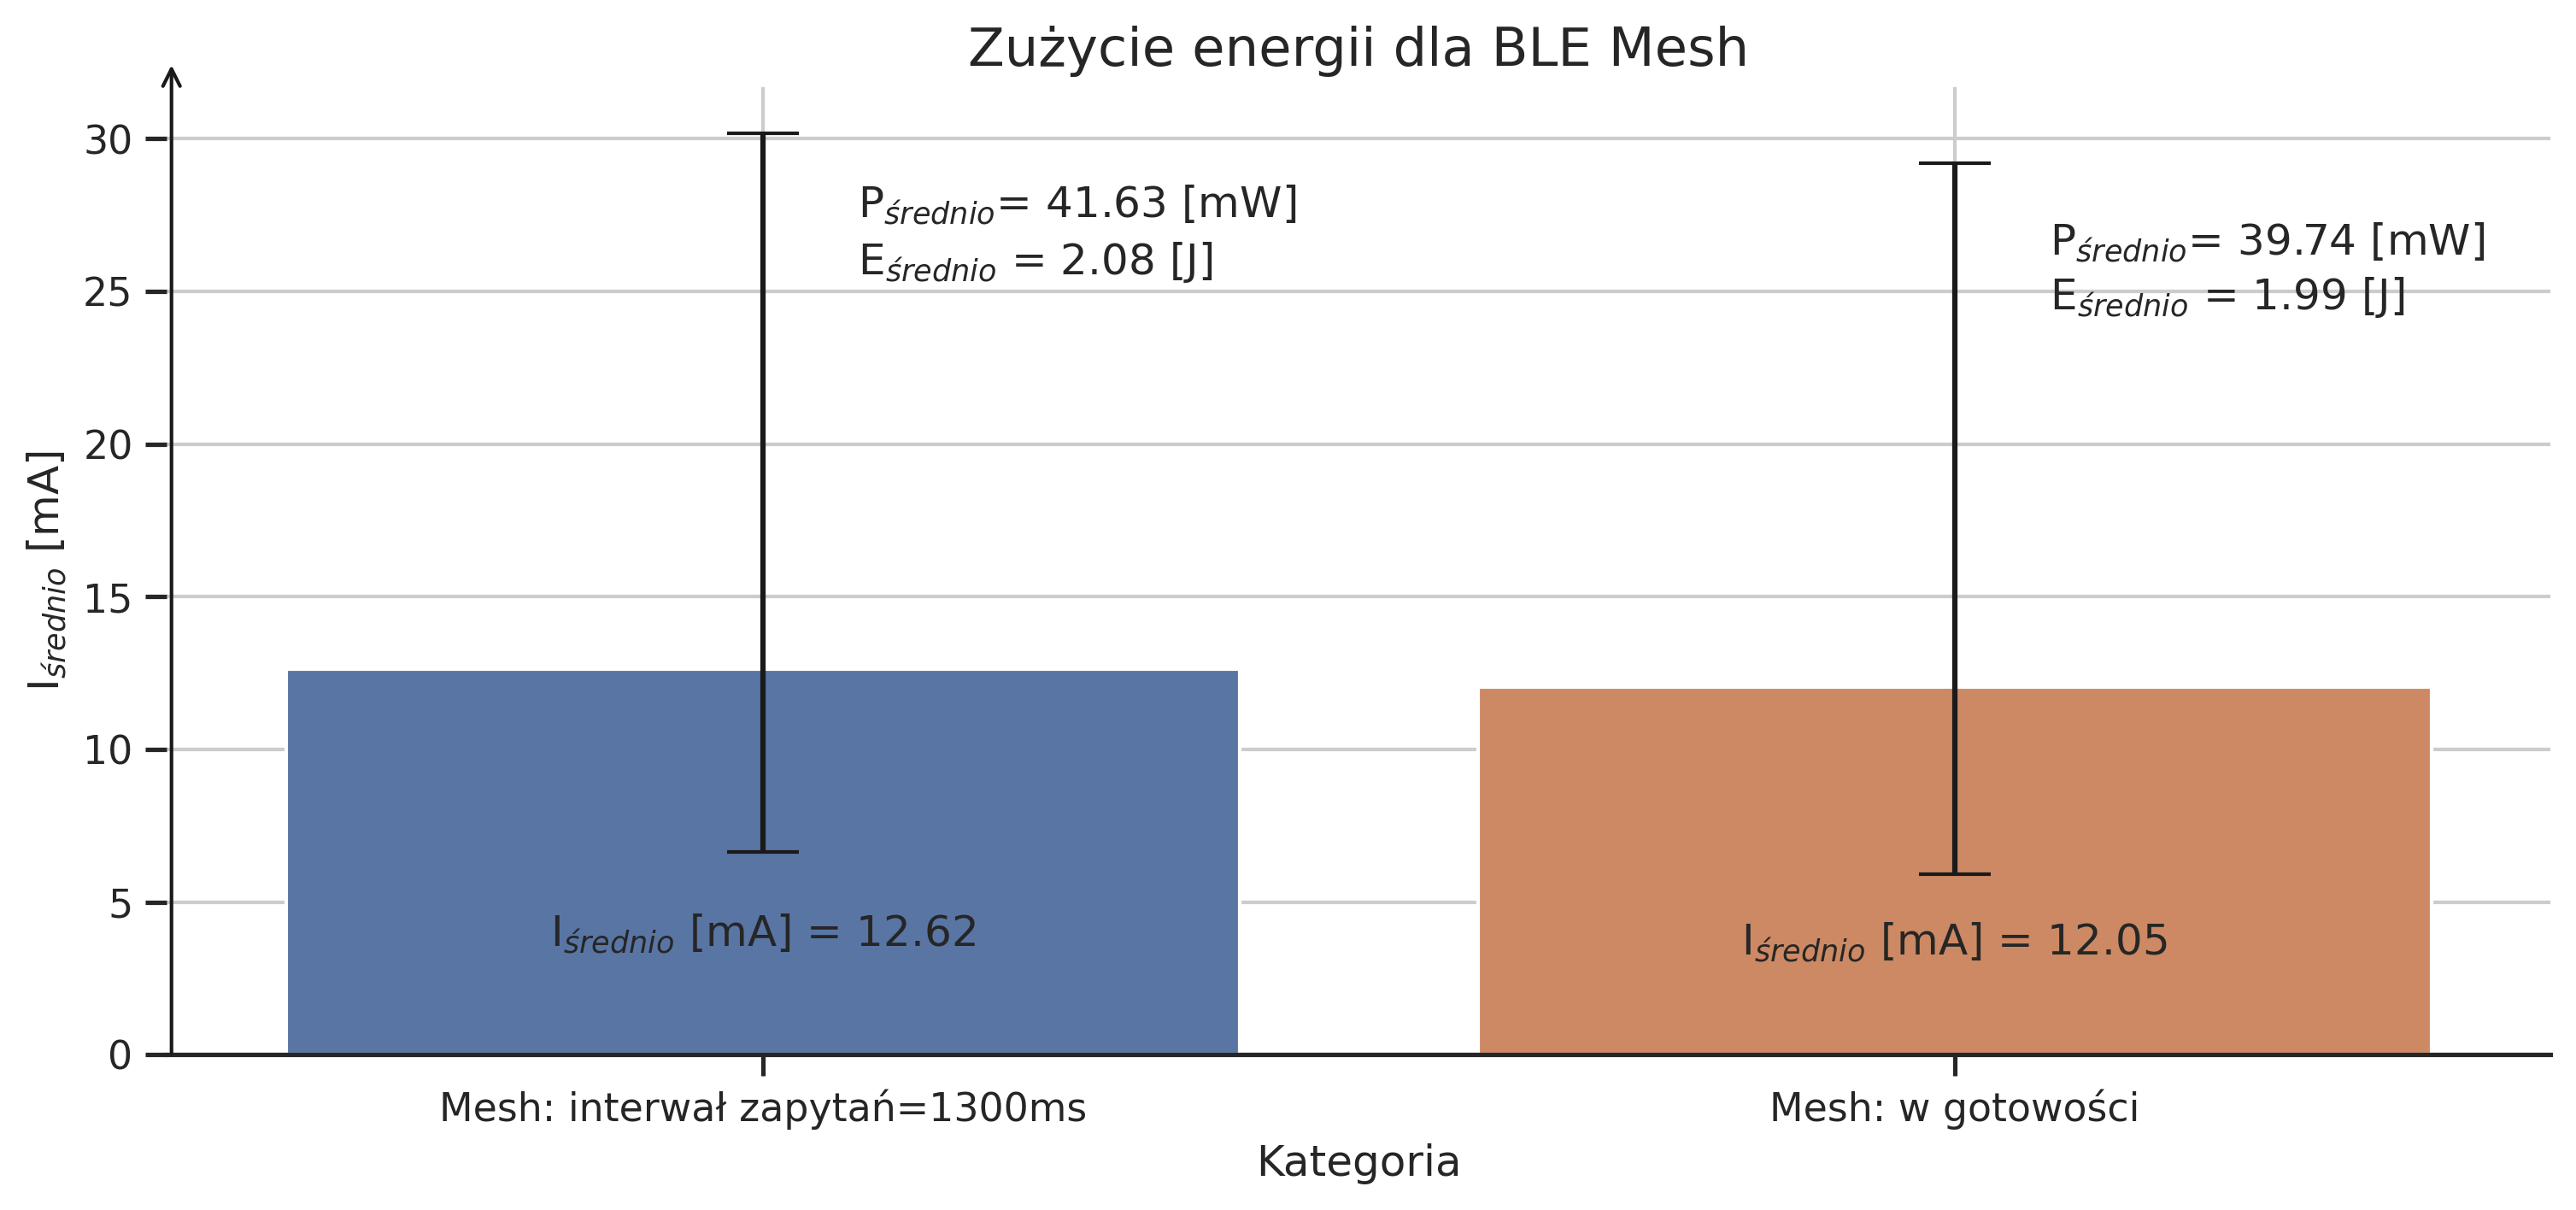
\includegraphics[width=0.99\linewidth]{power_ble_mesh_amps_usage_juxtaposition.png} 
	\caption{Zestawienie zużycia prądu dla BLE Mesh w zależności od trybu działania}
	\label{rys:power_ble_mesh_amps_usage_juxtaposition}
\end{figure}

\lipsum[1-3]
\begin{figure}[!htb]
	\centering 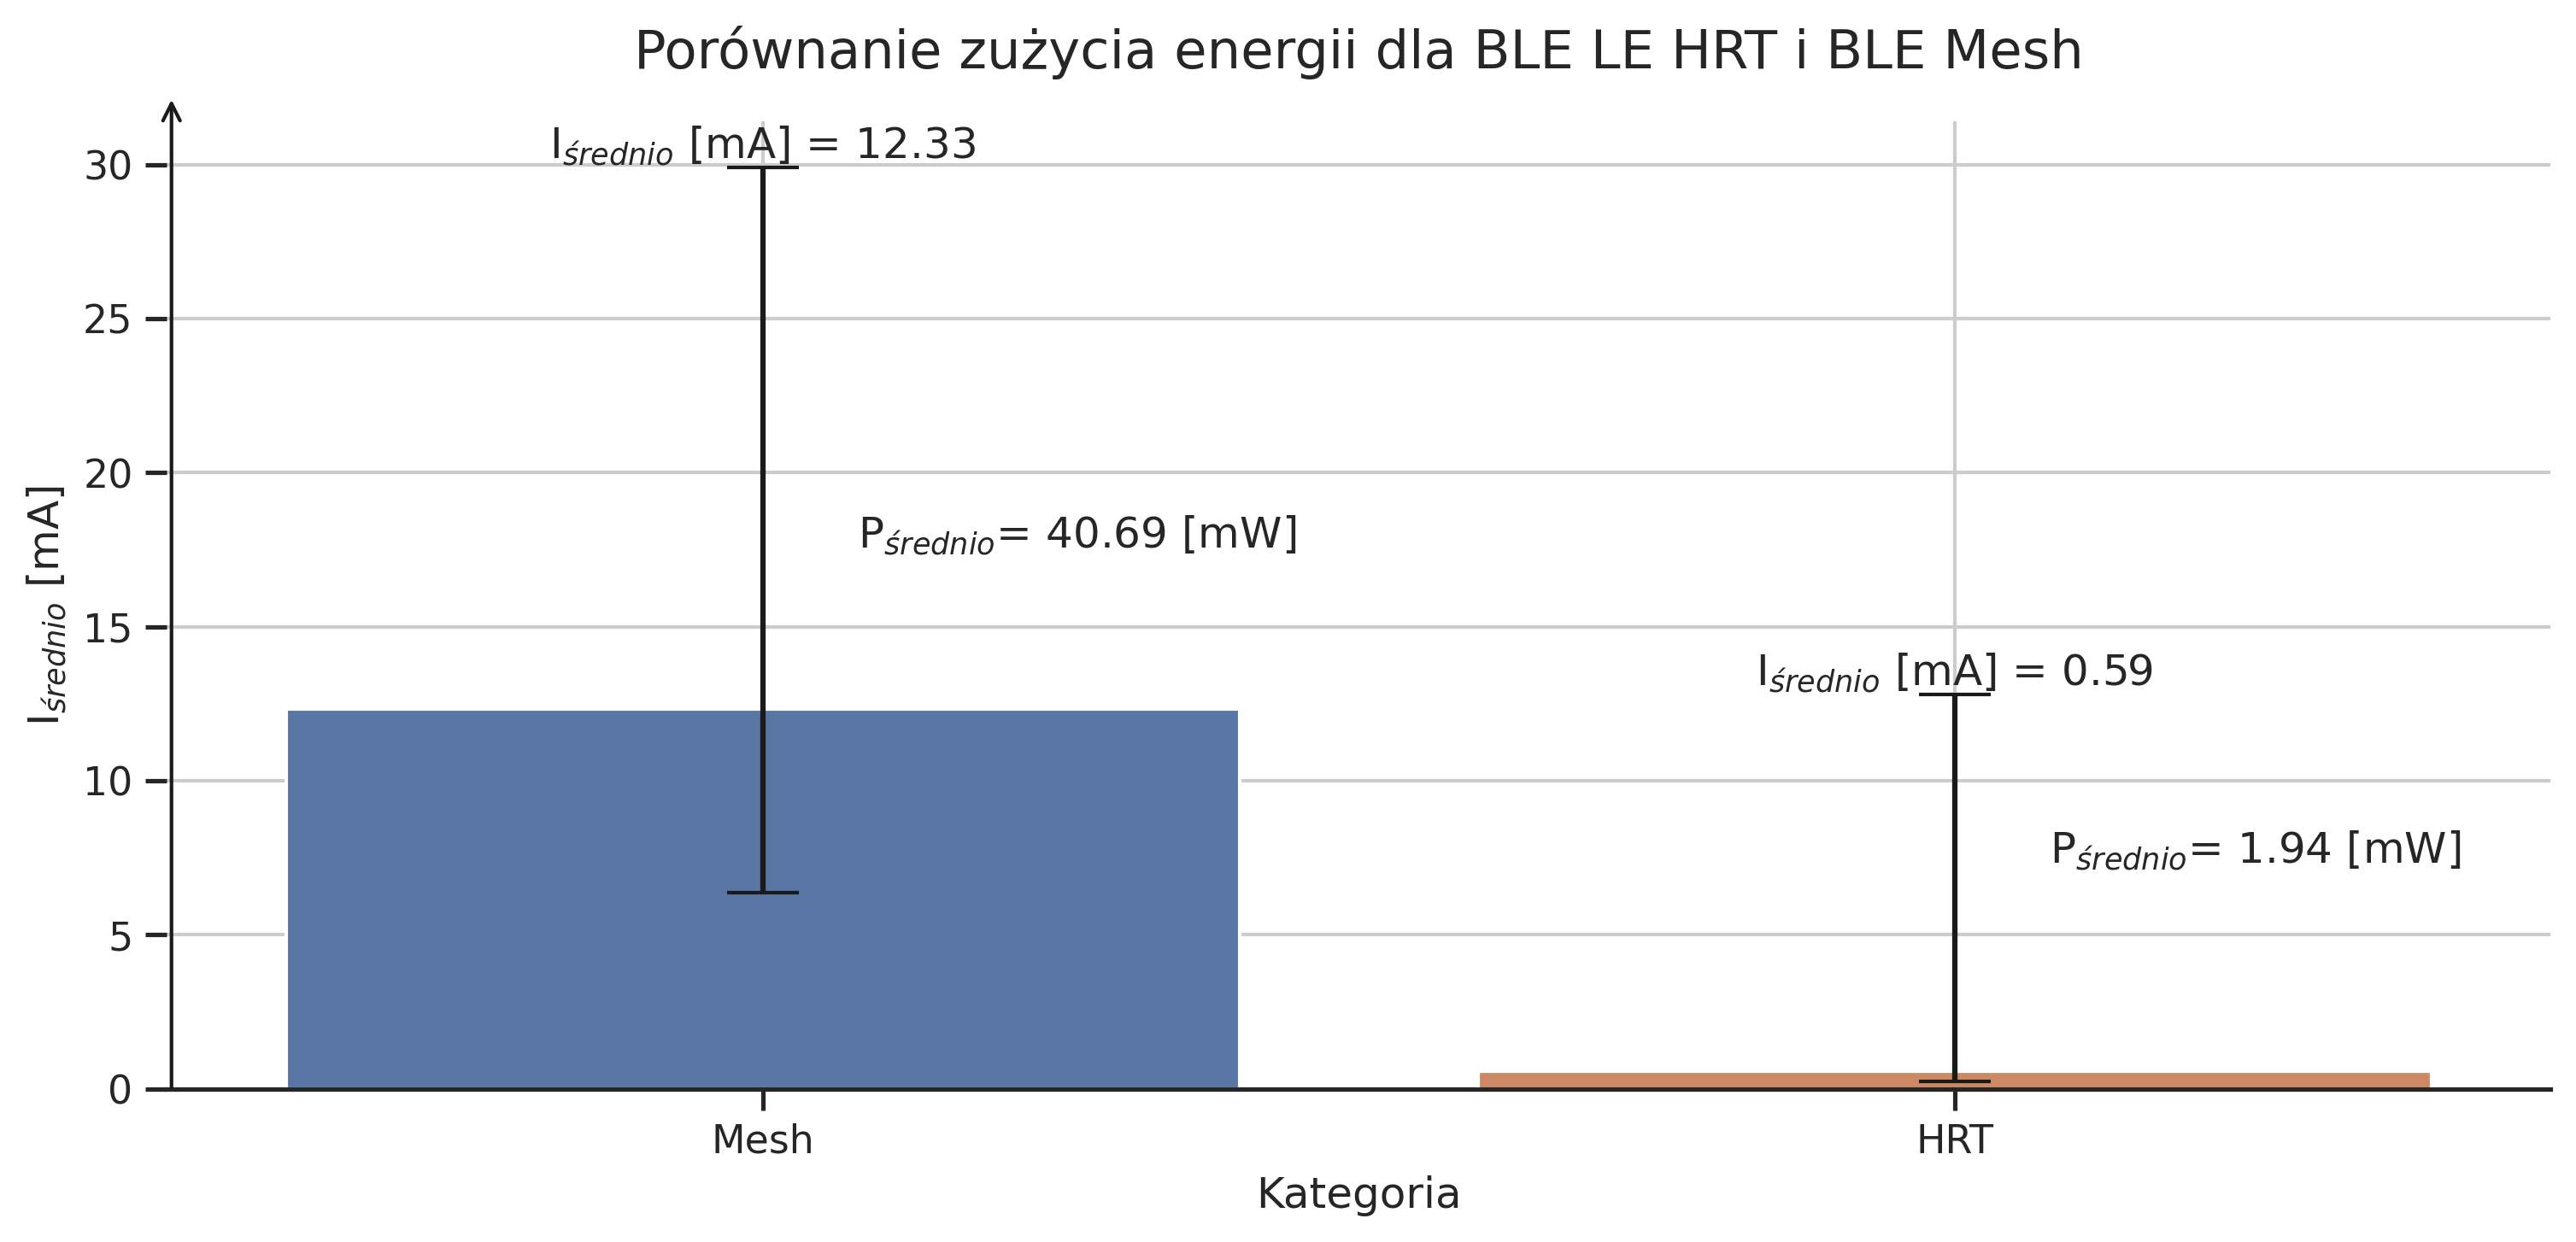
\includegraphics[width=0.99\linewidth]{power_ble_consumption_comparison.png} 
	\caption{Porównanie średniego zużycia energii pomiędzy BT Low Energy HRT i BLE Mesh}
	\label{rys:power_ble_consumption_comparison}
\end{figure}



%%!!!!!!!!!!!!!!!!!!!!!!!!!!!!!!!!!!!!!!!!!!!!!!!!!!!!!!!!!!!!!!!!!!!!!!!!!!!!!!
%%%%%%%%%%%%%%%%%%%%%%%%%%%%%%%%%%%%%%%%%%%%%%%%%%%%%%%%%%%%%%%%%%%%%%%%%%%%%%%%
%% SECTION: Packet Error Rate
%%%%%%%%%%%%%%%%%%%%%%%%%%%%%%%%%%%%%%%%%%%%%%%%%%%%%%%%%%%%%%%%%%%%%%%%%%%%%%%%
%%!!!!!!!!!!!!!!!!!!!!!!!!!!!!!!!!!!!!!!!!!!!!!!!!!!!!!!!!!!!!!!!!!!!!!!!!!!!!!!
\section{Packet Error Rate}

Celem niniejszych badań jest prezentacja metodologii przeprowadzonego eksperymentu \gls{PER} 
w~konfiguracji Mesh oraz prezentacja i~omówienie otrzymanych rezultatów.

 
%%%%%%%%%%%%%%%%%%%%%%%%%%%%%%%%%%%%%%%%%%%%%%%%%%%%%%%%%%%%%%%%%%%%%%%%%%%%%%%%
%% SUBSECTION: Zależność PER względem odległości między węzłami
%%%%%%%%%%%%%%%%%%%%%%%%%%%%%%%%%%%%%%%%%%%%%%%%%%%%%%%%%%%%%%%%%%%%%%%%%%%%%%%%
\subsection{Metodologia badania}
\subsubsection{Definicja pakietu}
Przed przystąpieniem do badań należy precyzyjnie zdefiniować wykorzystywaną terminologię.

Pakietem nazywamy pojedynczą porcję danych przetwarzaną na poziomie warstwy sieciowej modelu ISO OSI \cite{sa_tcpip_nodate}.
Warstwa ta umożliwia routing, adresowanie logiczne oraz przetwarzanie i~dostarczanie pakietów.

\begin{figure}[!ht]
	\centering 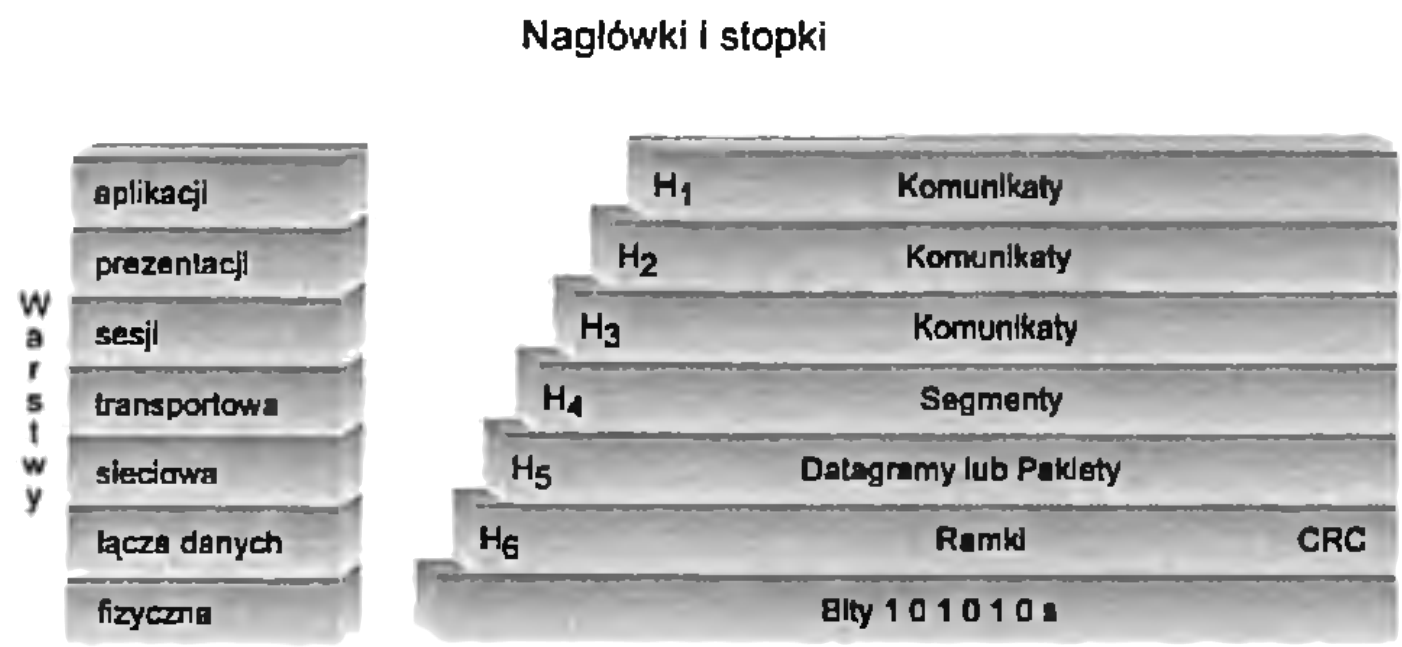
\includegraphics[width=0.618\linewidth]{tcp_ip_szkola_programowania_naglowki_stopki.png} 
	\caption{Model ISO OSI wraz i odpowiadające mu nazwy porcji danych. Źródło: \cite{sa_tcpip_nodate}}
	\label{rys:iso_osi_model_nazwy_grup_danych}
\end{figure}

\gls{BLE} wprowadza własną nomenklaturę dla poszczególnych warstw sieciowych. Jest to o tyle istotne, iż standard ten
nie zapewnia odpowiadających modelowi ISO OSI warstw jeden-do-jednego. Część z tych warstw jest agregowanych w~zespół 
protokołów wyższych warstw - Rysunek~\ref{rys:agregacja_protokolow_ble}. 

Bazując na definicji modelu OSI oraz stosie BLE, pakietem można nazwać wiadomości będące możliwie blisko
warstwy \textit{\gls{LL}}. Podobną definicję prezentuje dokumentacja ST:
\enquote{Pakiet to pojedyncza oznaczona wiadomość wysłana przez jedno i~odebrana przez 
co najmniej jedno urządzenie.}\footnote{Tłumaczenie własne}~\cite{stmicroelectronics_pm0271_2021}

\begin{figure}[!ht]
	\centering 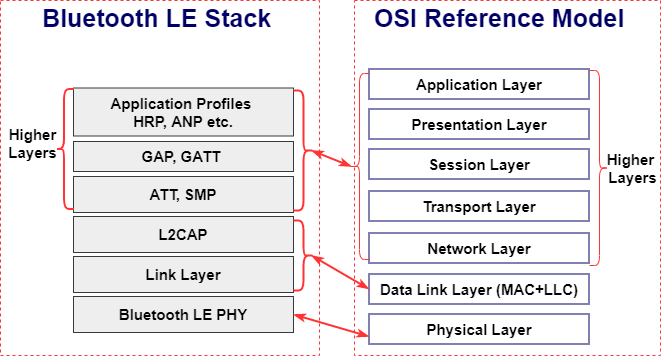
\includegraphics[width=0.618\linewidth]{mathworks_iso_osi_ble_stack.png} 
	\caption{Zestawienie stosu BLE i modelu ISO OSI. Źródło: \cite{noauthor_bluetooth_nodate}}
	\label{rys:agregacja_protokolow_ble}
\end{figure}

BLE Mesh dodatkowo wprowadza własne dodatkowe warstwy komunikacji, biorąc za podstawę stos BLE~\cite{mesh_working_group_mesh_2019}.
Każda z wymienionych warstw jest hermetyzowana za pośrednictwem dostarczanego przez producenta \gls{API}.
Uwzględniając zamknięcie middleware'u i dwu-procesorową architekturę mikrokontrolera STM32WB55, oznacza 
to brak możliwości bezpośredniego nasłuchiwania pakietów w~warstwie \gls{LL}.

Uwzględniając powyższe czynniki, pakietem dla BLE Mesh nazywana będzie wiadomość najbliższa warstwie \gls{LL}.
W przypadku stworzonego oprogramowania, oznacza to odbiór komunikatu odebranego jako zdarzenie zarejestrowane przez
koprocesor Cortex-M0, będący integralną częścią mikrokontrolera STM32WB55 odpowiadający za obsługę radia.

\subsubsection{Definicja Packet Error Rate}
Posiadając definicję pakietu, \gls{PER} definiuje się następująco: PER jest miarą ilości błędnych pakietów w proporcji do 
wszystkich wysłanych pakietów, zgodnie ze wzorem:

\begin{equation}
PER = \frac{s - r}{s} \cdot 100\%
\end{equation}
gdzie:
\begin{description}
\item[s] is ilość wysłanych pakietów
\item[r] is ilość odebranych pakietów
\item[s-r] - ilość niepoprawnych/błędnych pakietów
\end{description}

\subsubsection{Procedura badawcza}

(Jakiś mały akapit wstępu...)

Stałe parametry transmisji danych:
\begin{itemize}
\item Szybkość transmisji: 2Mbps
\item Moc transmisji danych: 0dBm
\end{itemize}


Eksperyment wyznaczający PER oparto o następujące czynniki zmienne:
\begin{itemize}
\item środowisko: teren leśny, teren zurbanizowany
\item interwał zapytań
\item dystans pomiędzy węzłami
\item ilość węzłów składających się na sieć Mesh
\end{itemize}

Wyznaczanie PER odbyło się w dwóch różnych środowiskach. Jednym z głównych hipotez jest znaczący wpływ
środowiska na jakość transmisji danych. Czynniki takie jak temperatura, wilgotność, rodzaj gleby czy
tło radiowe może mieć wpływ na komunikację pomiędzy węzłami. Założono, iż tło radiowe może mieć
największy wpływ ja transmisję danych. Stąd dobrano możliwie skrajne miejsca do badań oceniając
to jako najistotniejszy czynnik:
\begin{itemize}
\item Kampinowski Park Narodowy (lokalizacja: parking Roztoka) - jako teren leśny oddalony od ośrodka miejskiego
ze względnie niewielkim tłem radiowym. Pogoda: pochmurnie, wilgotno, temperatura poniżej 20$^{\circ}$C.
\item Park Pola Mokotowskie - jako teren zurbanizowany charakteryzujący się bogatym tłem radiowym działającym
w pasmach \gls{ISM}. Pogoda: słonecznie, temperatura ok. 20$^{\circ}$C.
\end{itemize}

Kolejnym badanym czynnikiem jest interwał zapytań. Parametr ten został wybrany ze względu na obserwowane
problemy z komunikacją podczas etapu tworzenia oprogramowania. Parametry dobrano w takim stopniu, by ów problem
ukazać. Obrano następujące interwały:
\begin{itemize}
\item 100ms
\item 500ms
\item 800ms
\item 1300ms
\item 2100ms
\end{itemize}

Interesującym parametrem dla bezprzewodowej transmisji danych jest zasięg. Stąd też, jednym z badanych czynników jest
określenie jakości PER w zależności od odległości - Rysunek~\ref{rys:two_nodes_setup}.
\begin{itemize}
\item 1,5m
\item 3,0m
\item 5,0m
\item 8,0m
\item 13,0m
\item 16,0m
\item 21,0m
\end{itemize}

\begin{figure}[!ht]
	\centering 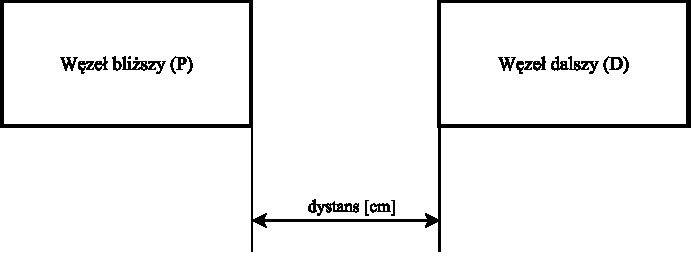
\includegraphics[width=0.618\linewidth]{per_two_nodes.pdf} 
	\caption{Dystans pomiędzy węzłami dla sieci dwóch mikrokontrolerów}
	\label{rys:two_nodes_setup}
\end{figure}

Wyżej wymienione odległości stosowano również w przypadku kolejnego badanego parametru, tj. ilości węzłów
składających się na sieć BLE. W celu łatwej identyfikacji węzłów, wprowadza się następujące nazewnictwo:
\begin{itemize}
	\item węzeł bliższy (ang./łac. \textit{proximal node}/\textit{nodus proximalis}) - węzeł będący połączony bezpośrednio
	ze stacją akwizycji danych i kontroli przepływu eksperymentu.
	\item węzeł środkowy (ang./łac. \textit{intermedial node}/\textit{nodus [inter]medius}) - węzeł działający w trybie
	przekaźnika (terminologia Mesh: \textit{Relay}). Węzeł ten nie uczestniczy bezpośrednio w badaniach tj. nie są
	z niego odczytywane jakiekolwiek dane.
	\item węzeł dalszy (ang./łac. \textit{distal node}/\textit{nodus distalis}) - węzeł zliczający ilość odebranych danych \textit{r},
	udostępniający jednocześnie usługę umożliwiającą odczyt tych wartości tak jak opisano to w podrozdziale \ref{prep:uc-software}.
\end{itemize}

Postanowiono o równoodległym rozstawieniu węzłów - Rysunek~\ref{rys:three_nodes_setup}. Dla sieci 3 węzłów,
maksymalna odległość dzieląca węzeł bliższy od węzła dalszego to 42m. Protokół badawczy zawiera informację 
tylko o odległości w~rozumieniu równoodległego rozstawienia węzłów. Odległość pomiędzy elementami 
jest oczywistą operacją arytmetyczną.

\begin{figure}[!ht]
	\centering 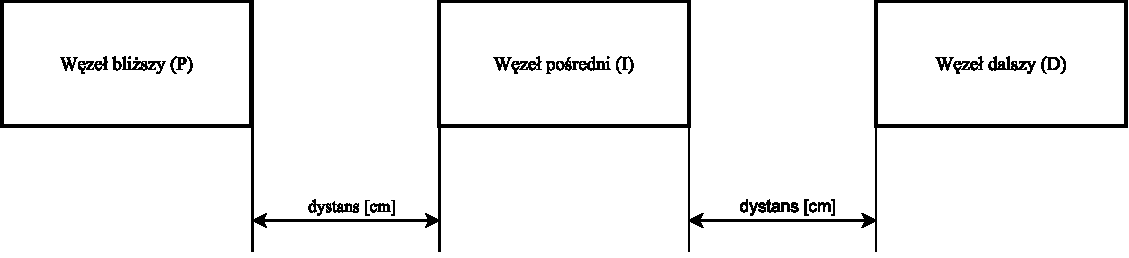
\includegraphics[width=0.99\linewidth]{per_three_nodes.pdf} 
	\caption{Dystans pomiędzy węzłami dla sieci trzech mikrokontrolerów}
	\label{rys:three_nodes_setup}
\end{figure}

Odległość pomiędzy węzłami mierzona jest z użyciem taśmy mierniczej z podziałką 1mm. Tolerancję pomiarów należy
przyjąć jako najdłuższy wymiar zestawu uruchomieniowego P-NUCLEO-WB55 - 70mm \cite{stmicroelectronics_um2435_2019}.

%%%%%%%%%%%%%%%%%%%%%%%%%%%%%%%%%%%%%%%%%%%%%%%%%%%%%%%%%%%%%%%%%%%%%%%%%%%%%%%%
%% SUBSECTION: Zależność \gls{PER} względem częstości zapytań
%%%%%%%%%%%%%%%%%%%%%%%%%%%%%%%%%%%%%%%%%%%%%%%%%%%%%%%%%%%%%%%%%%%%%%%%%%%%%%%%
\subsection{Zależność PER względem częstości zapytań}

\begin{figure}[!htb]
	\centering 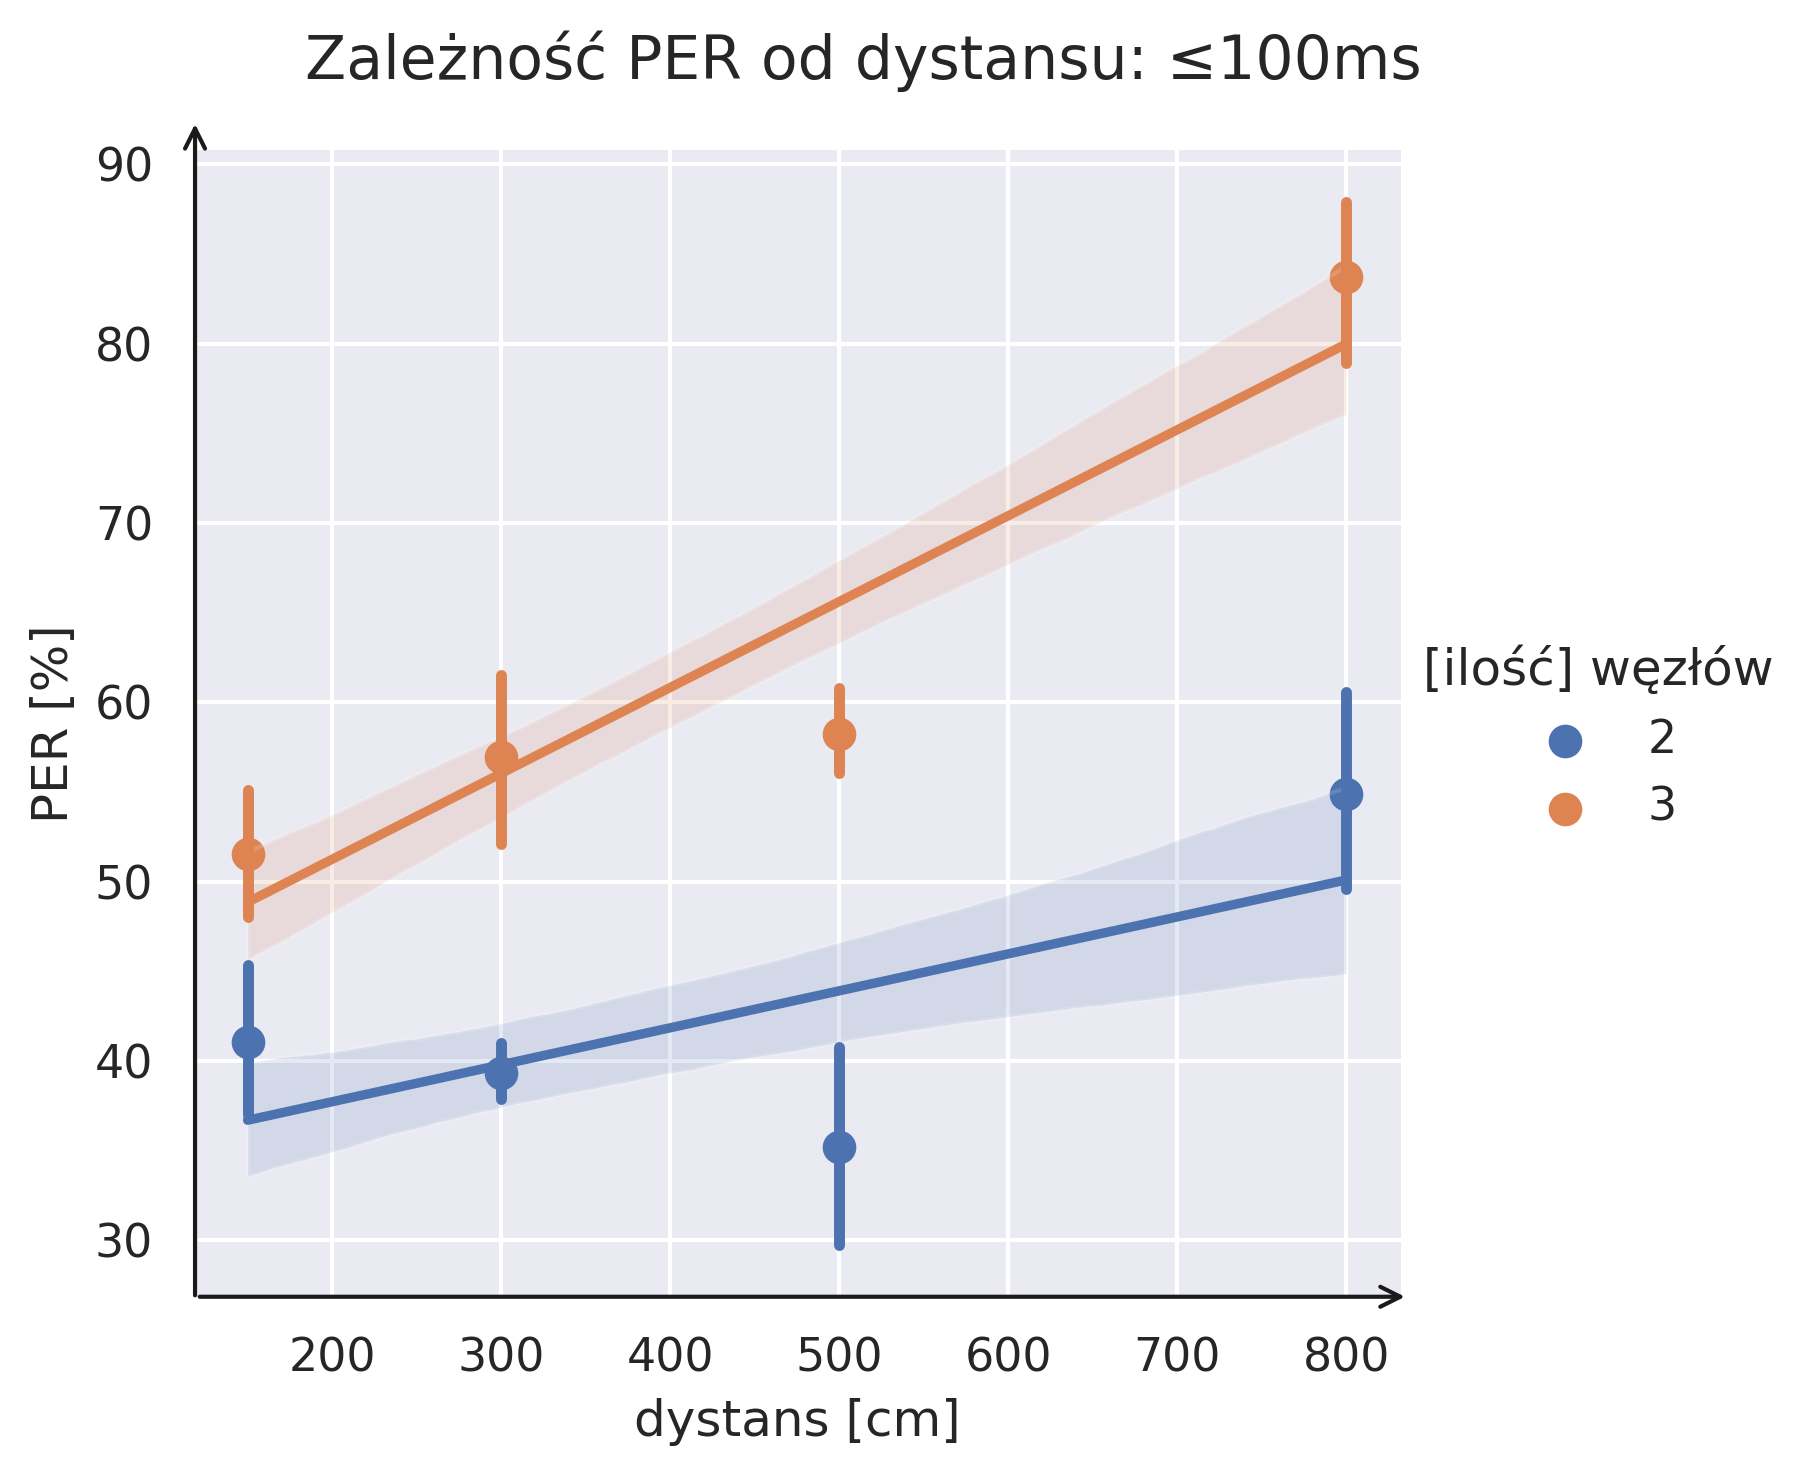
\includegraphics[width=0.618\linewidth]{per_to_distance_under_100ms.png}
	\caption{Zależność \gls{PER} od dystansu dla zapytań o częstości $\leqslant$ 100ms dla różnej liczby węzłów}
	\label{rys:per_to_distance_under_100ms}
\end{figure}

\begin{figure}[!htb]
	\centering 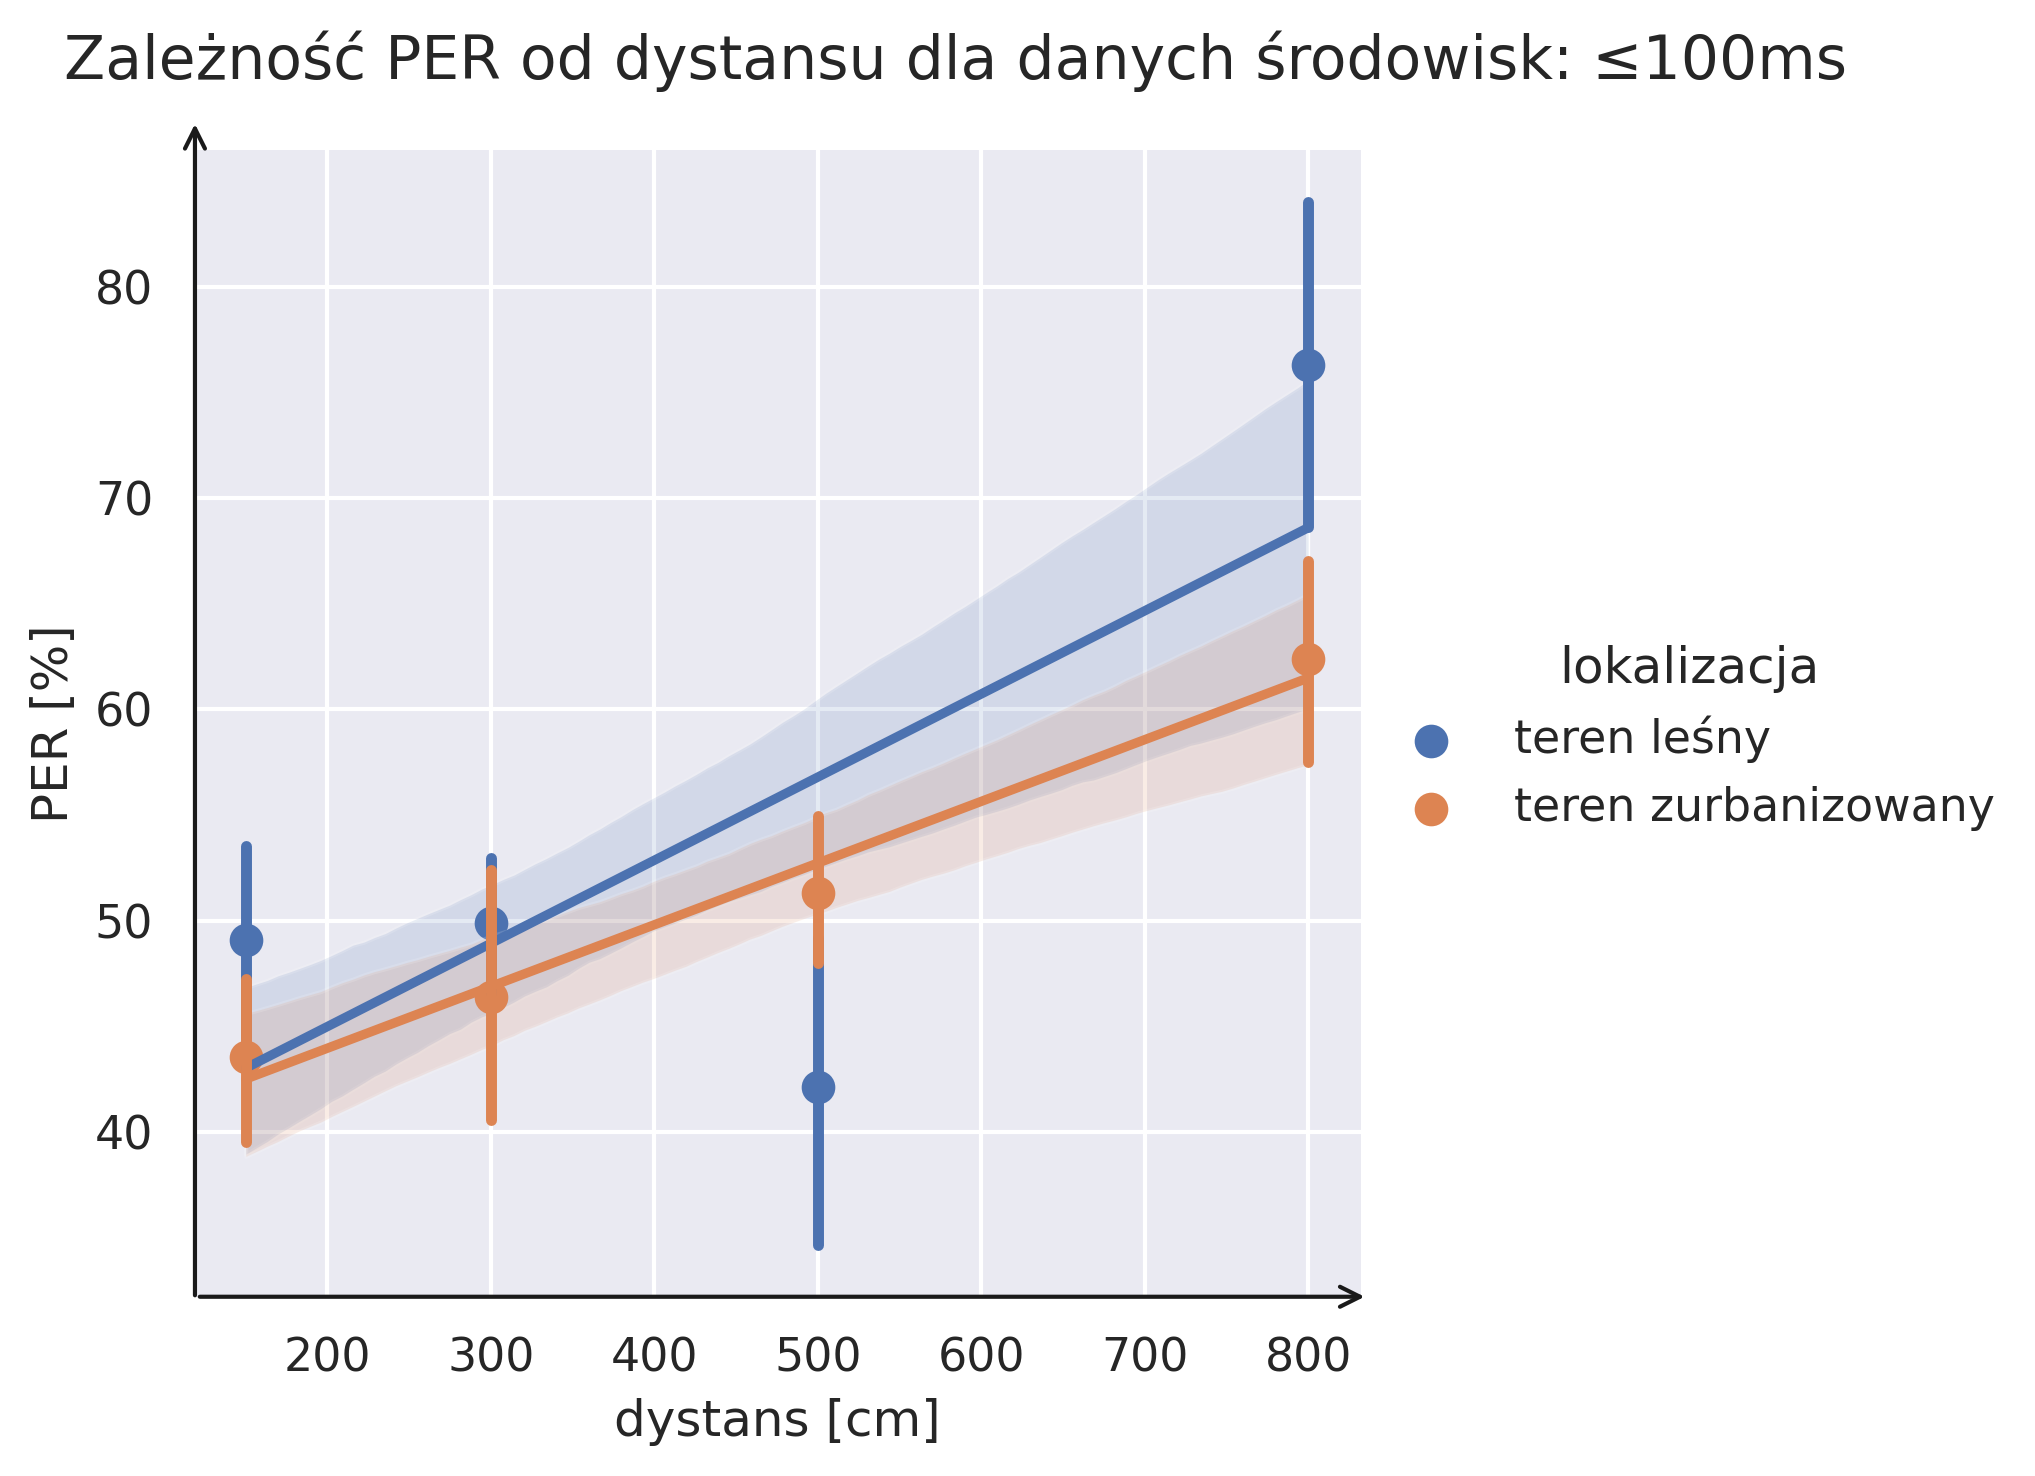
\includegraphics[width=0.618\linewidth]{per_to_distance_under_100ms_different_envs.png} 
	\caption{Zależność \gls{PER} od dystansu dla zapytań o częstości $\leqslant$ 100ms w wybranych środowiskach bez rozróżnienia na liczbę węzłów}
	\label{rys:per_to_distance_under_100ms_different_envs}
\end{figure}

\begin{figure}[!htb]
	\centering 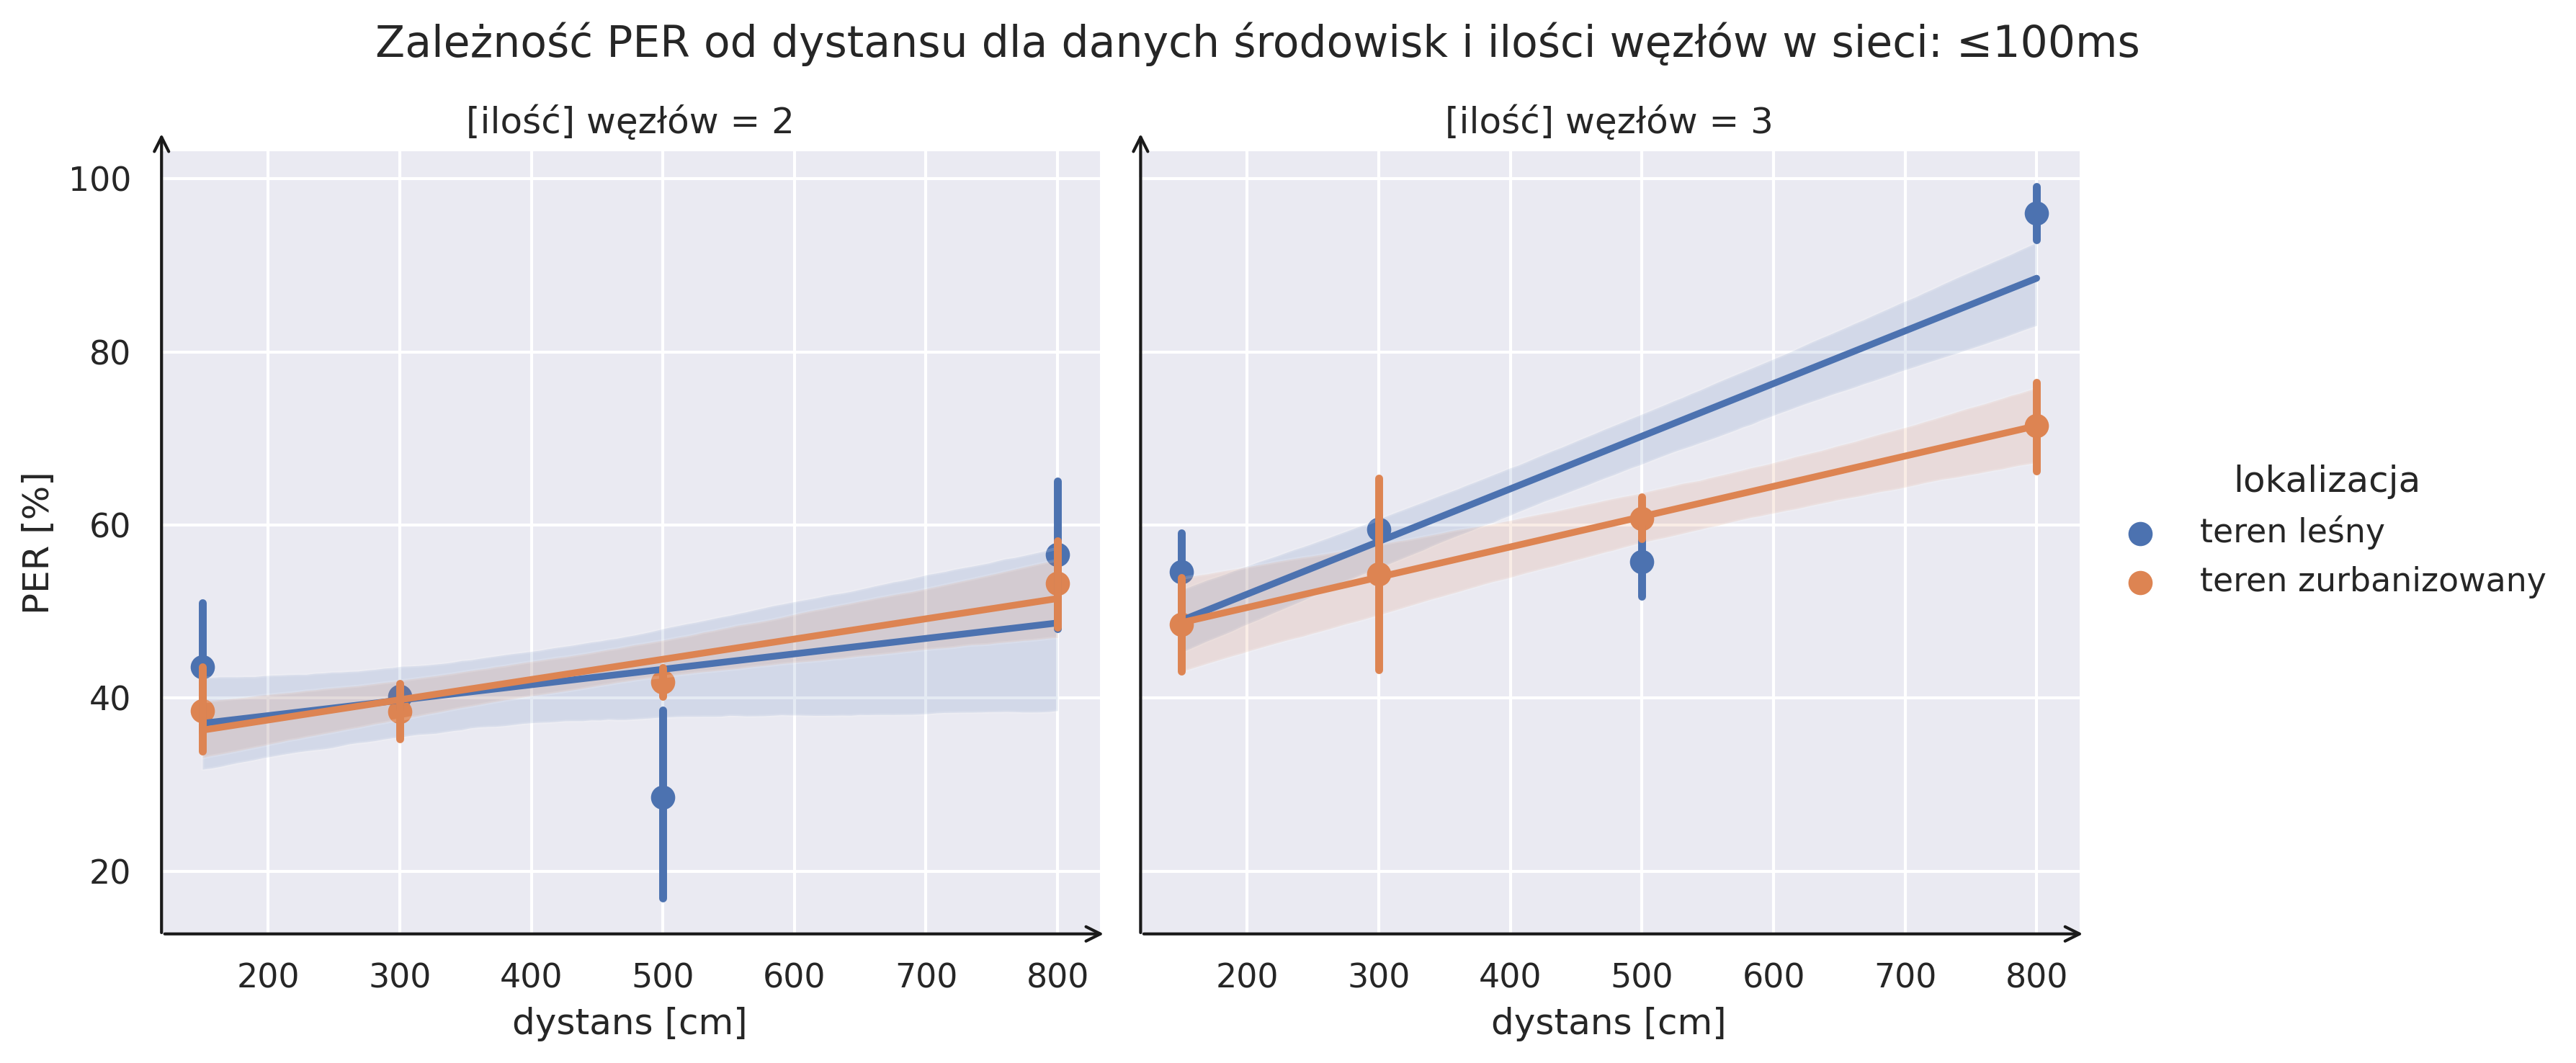
\includegraphics[width=0.99\linewidth]{per_to_distance_under_100ms_different_envs_and_nodes.png}
	\caption{Zależność \gls{PER} od dystansu dla zapytań o częstości $\leqslant$ 100ms w wybranych środowiskach i liczbę badanych węzłów}
	\label{rys:per_to_distance_under_100ms_different_envs_and_nodes}
\end{figure}

\begin{figure}[!htb]
	\centering 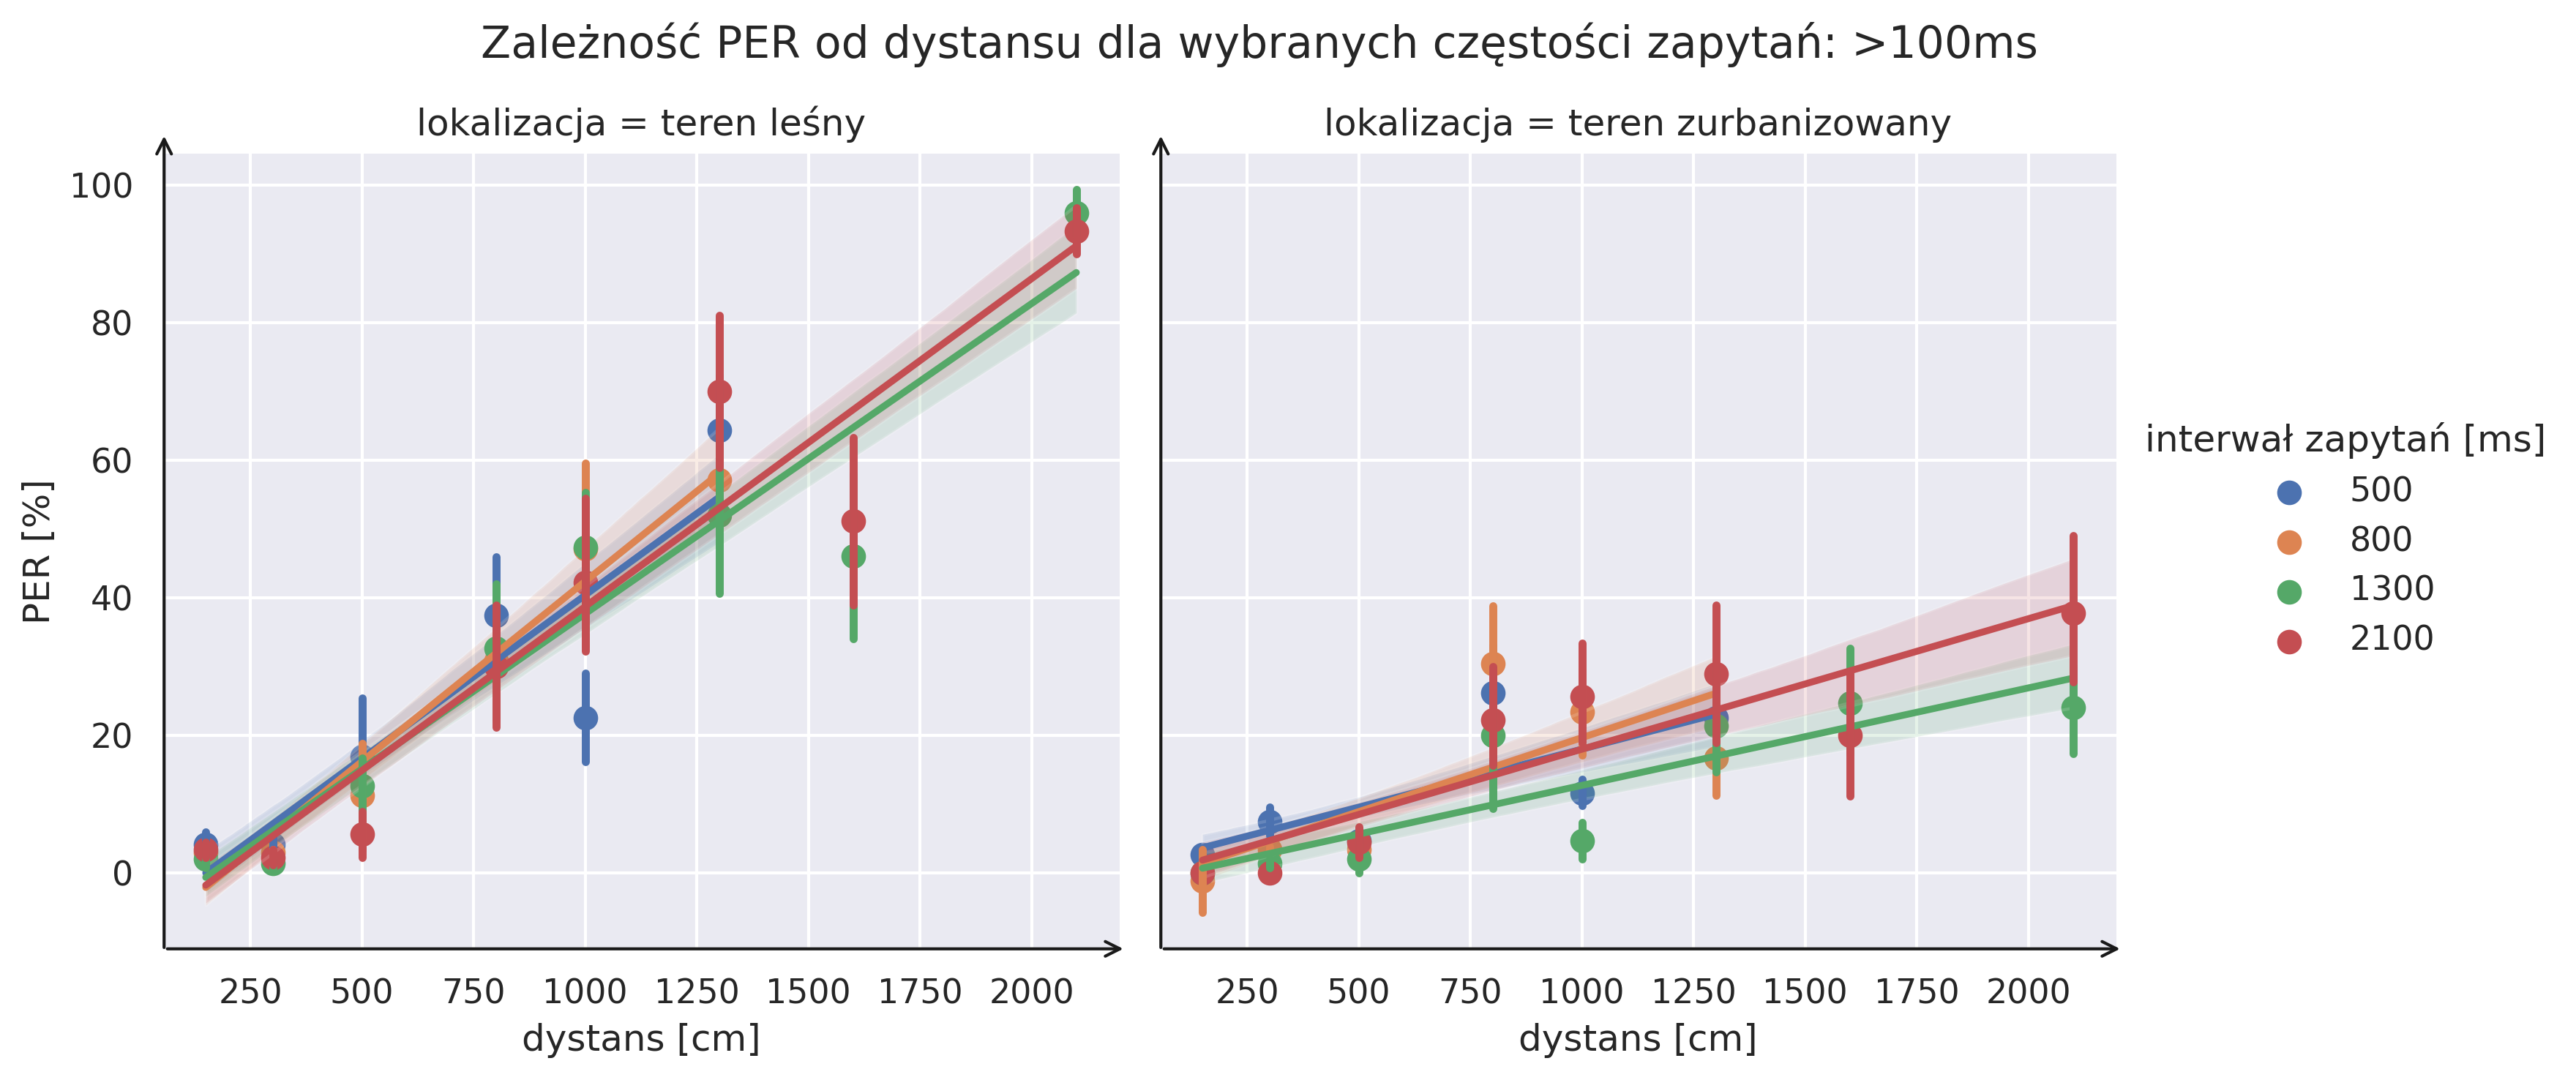
\includegraphics[width=0.99\linewidth]{per_to_distance_over_100ms_different_envs_different_ping_interval.png} 
	\caption{Zależność \gls{PER} od dystansu dla zapytań o częstości >100ms w wybranych środowiskach}
	\label{rys:per_to_distance_over_100ms_different_envs_different_ping_interval}
\end{figure}


%%%%%%%%%%%%%%%%%%%%%%%%%%%%%%%%%%%%%%%%%%%%%%%%%%%%%%%%%%%%%%%%%%%%%%%%%%%%%%%%
%% SUBSECTION: Zależność \gls{PER} względem odległości między węzłami
%%%%%%%%%%%%%%%%%%%%%%%%%%%%%%%%%%%%%%%%%%%%%%%%%%%%%%%%%%%%%%%%%%%%%%%%%%%%%%%%
\subsection{Zależność PER względem odległości między węzłami}

\begin{figure}[!htb]
	\centering 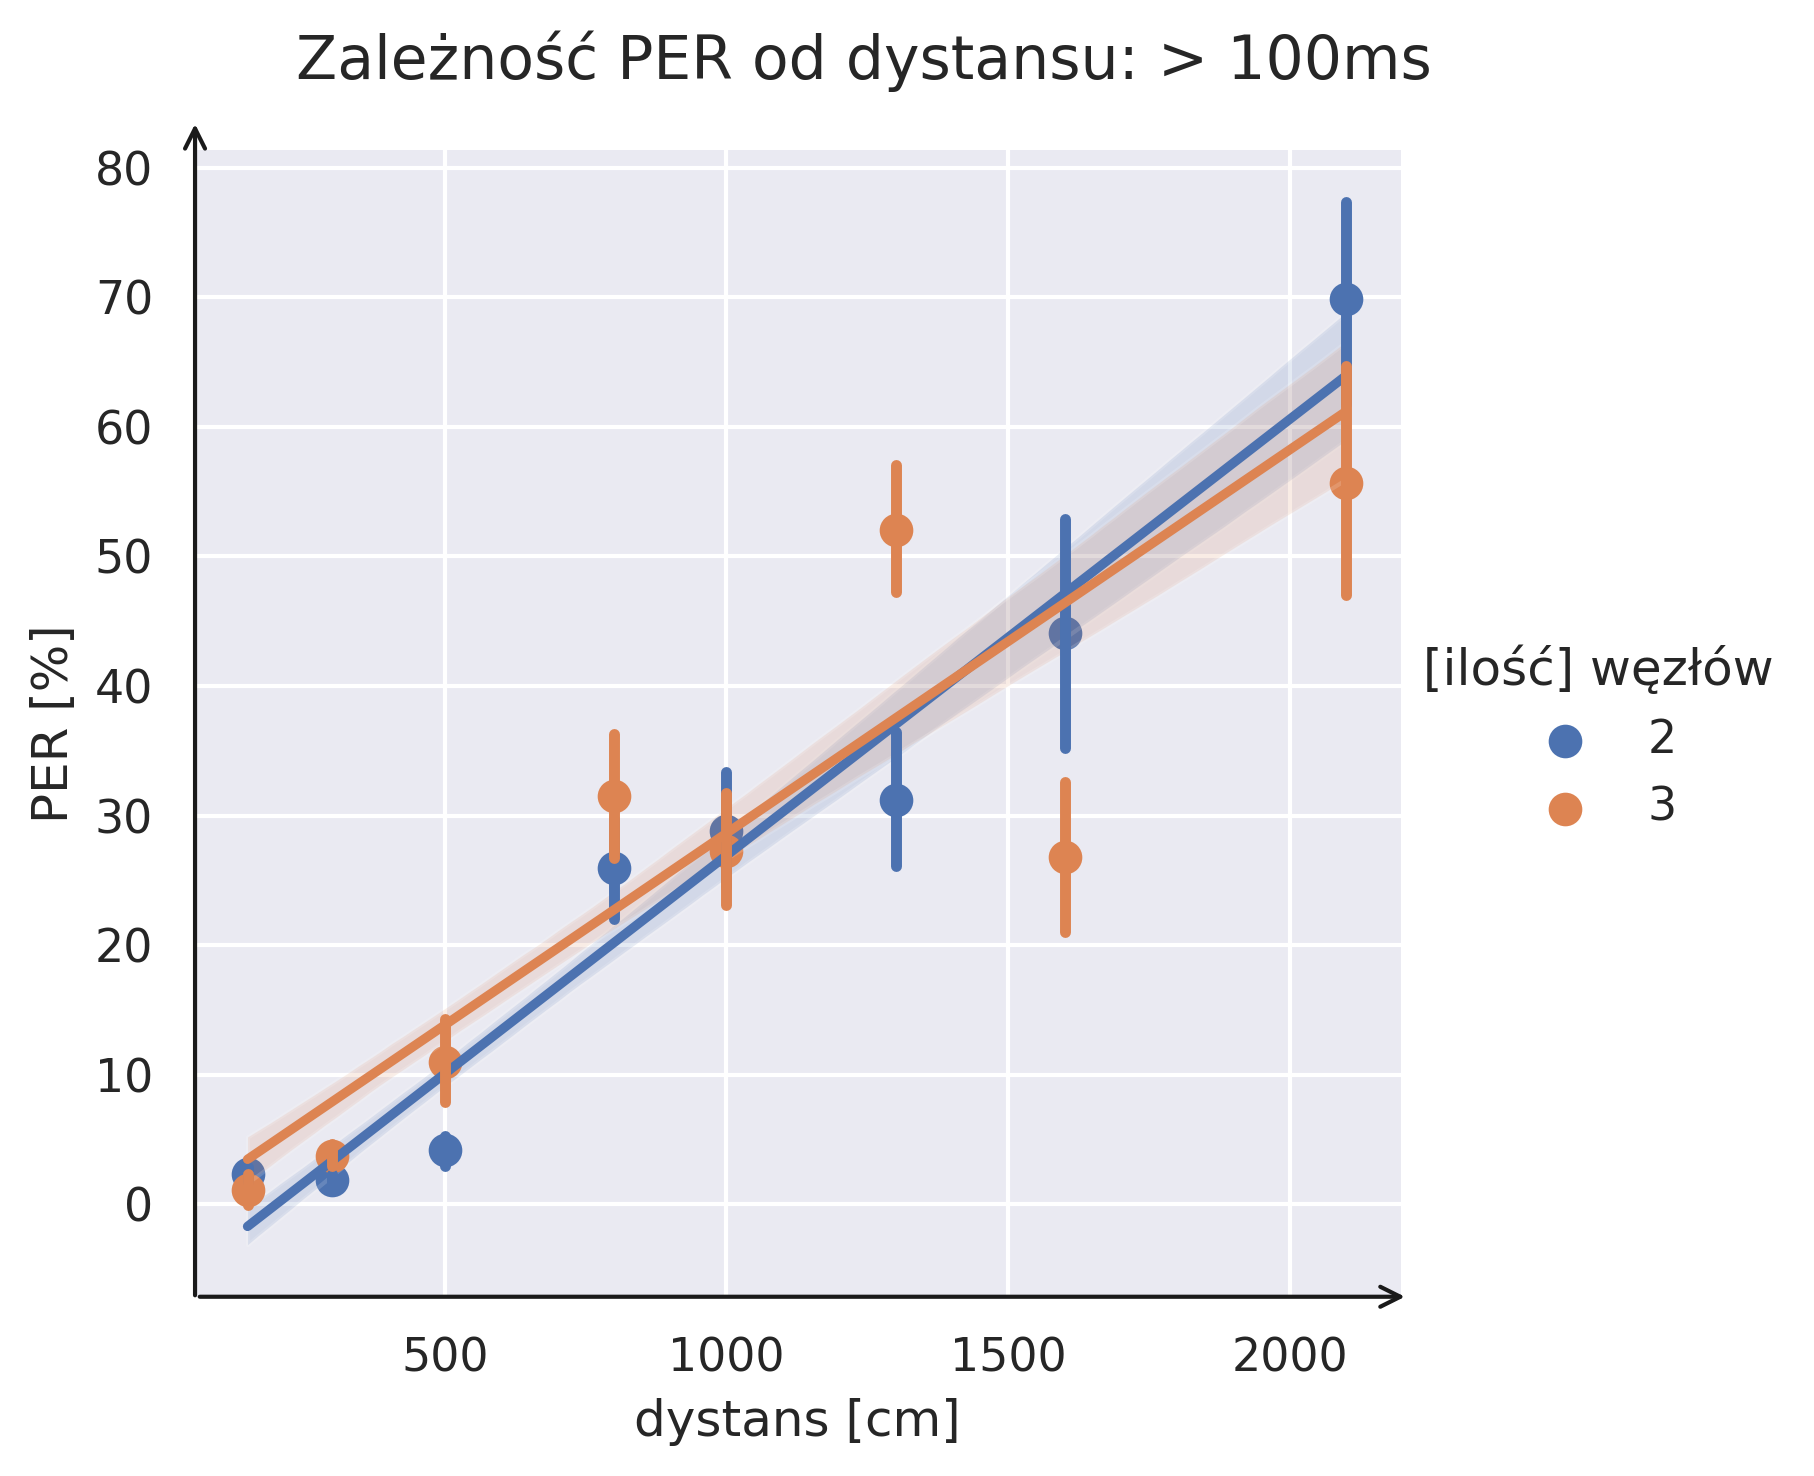
\includegraphics[width=0.618\linewidth]{per_to_distance_over_100ms.png}
	\caption{Zależność \gls{PER} od dystansu dla zapytań o częstości >100ms dla różnej liczby węzłów}
	\label{rys:per_to_distance_over_100ms}
\end{figure}

\begin{figure}[!htb]
	\centering 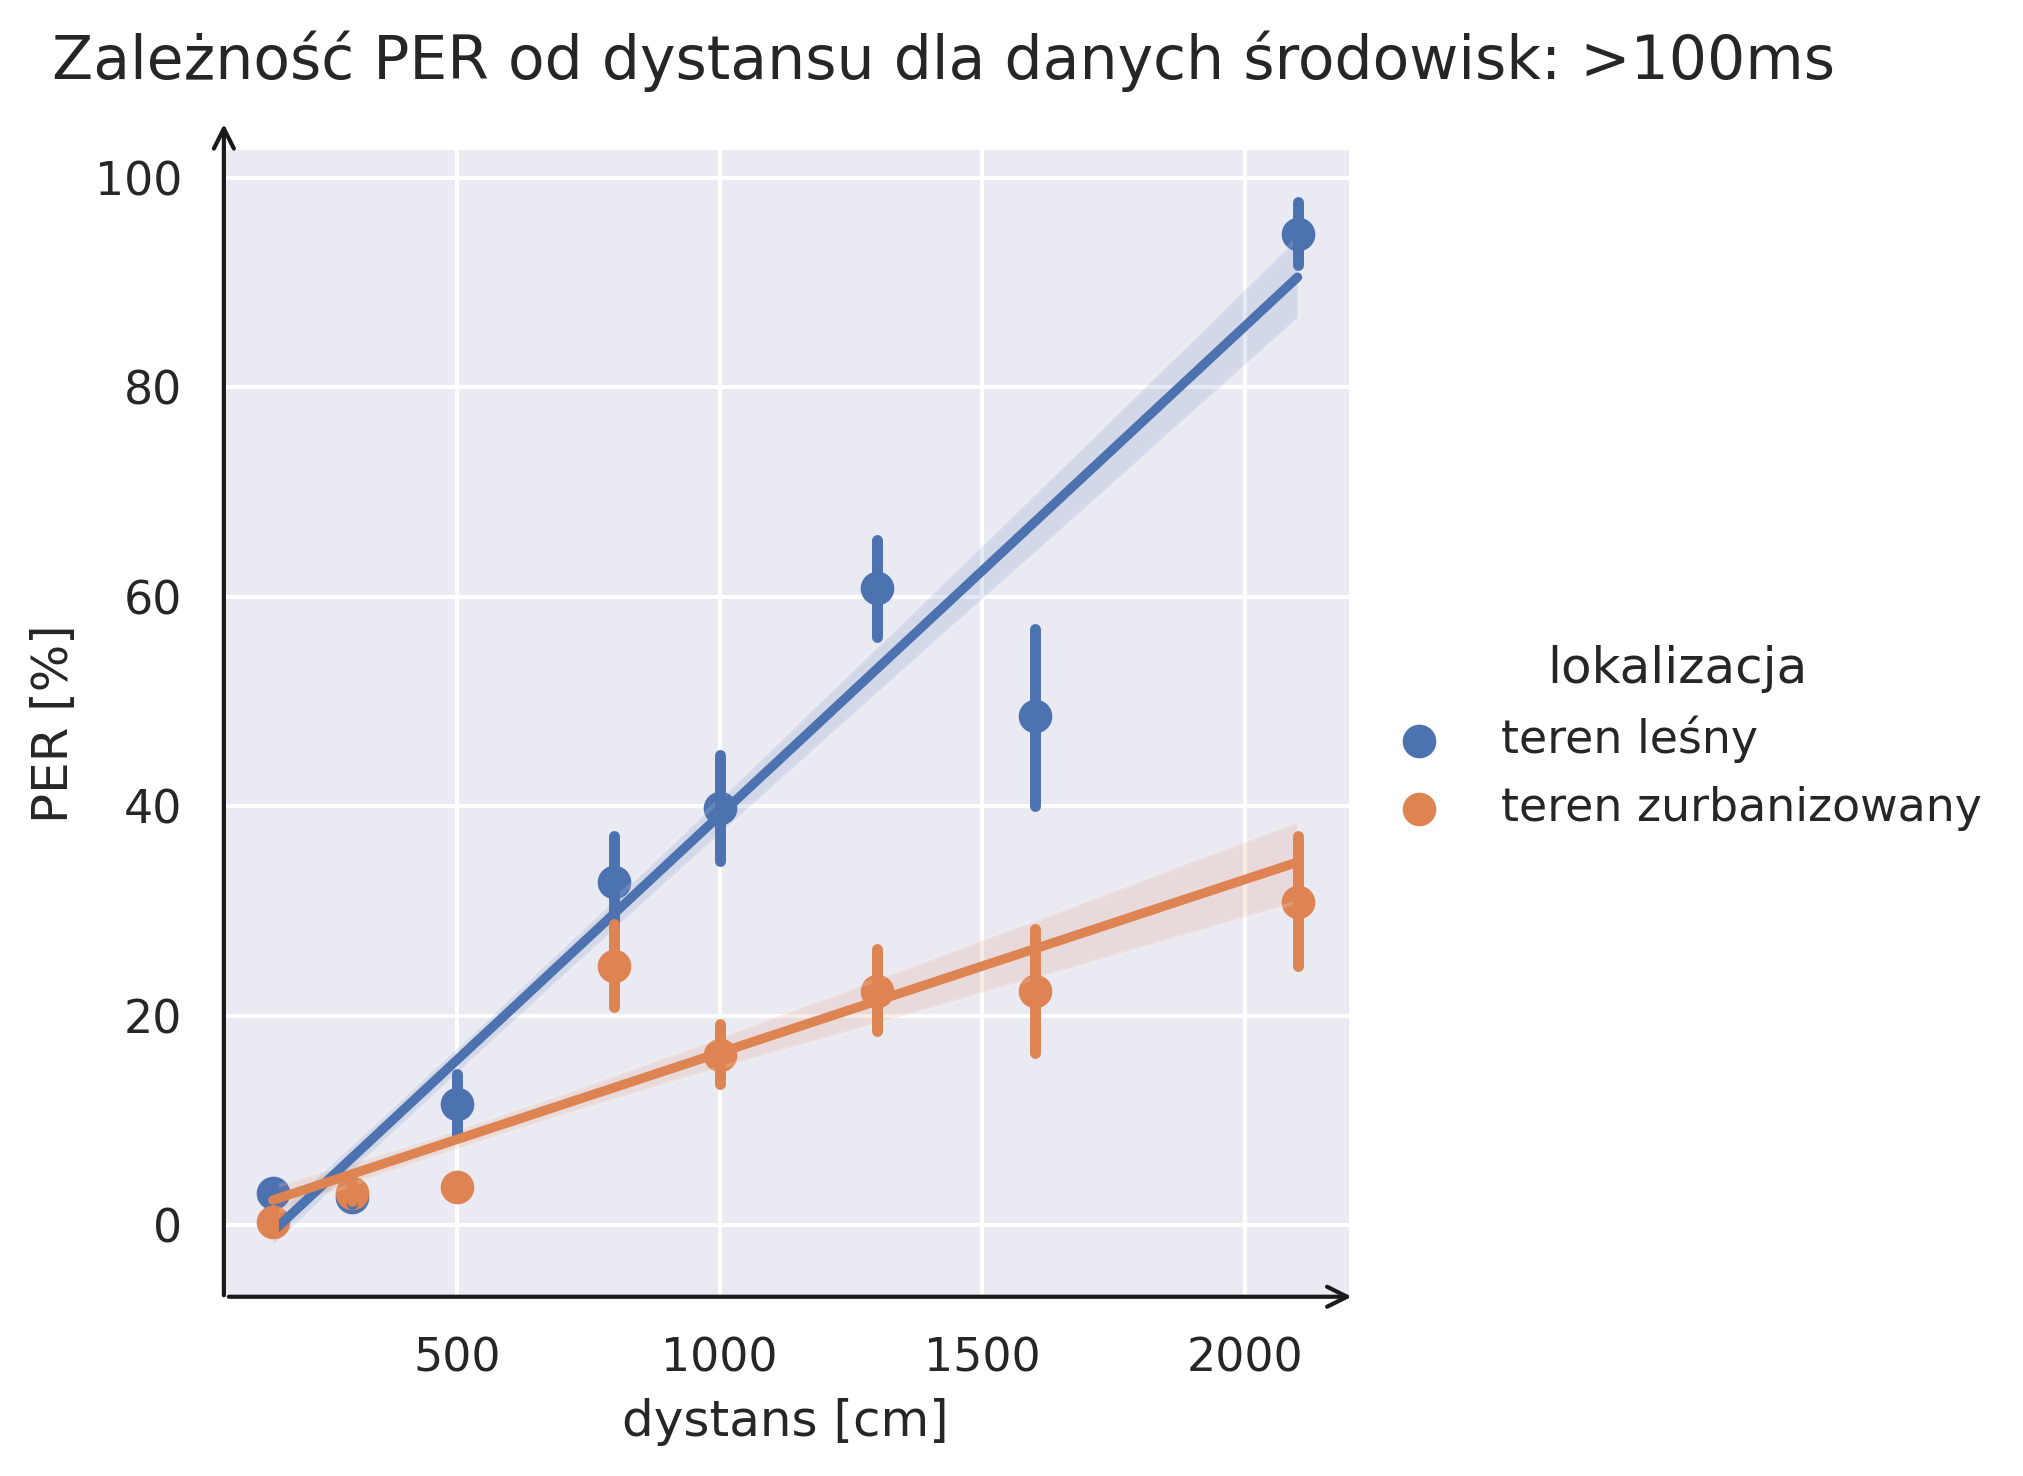
\includegraphics[width=0.618\linewidth]{per_to_distance_over_100ms_different_envs.png} 
	\caption{Zależność \gls{PER} od dystansu dla zapytań o częstości >100ms w wybranych środowiskach bez rozróżnienia na liczbę węzłów}
	\label{rys:per_to_distance_over_100ms_different_envs}
\end{figure}

\begin{figure}[!htb]
	\centering 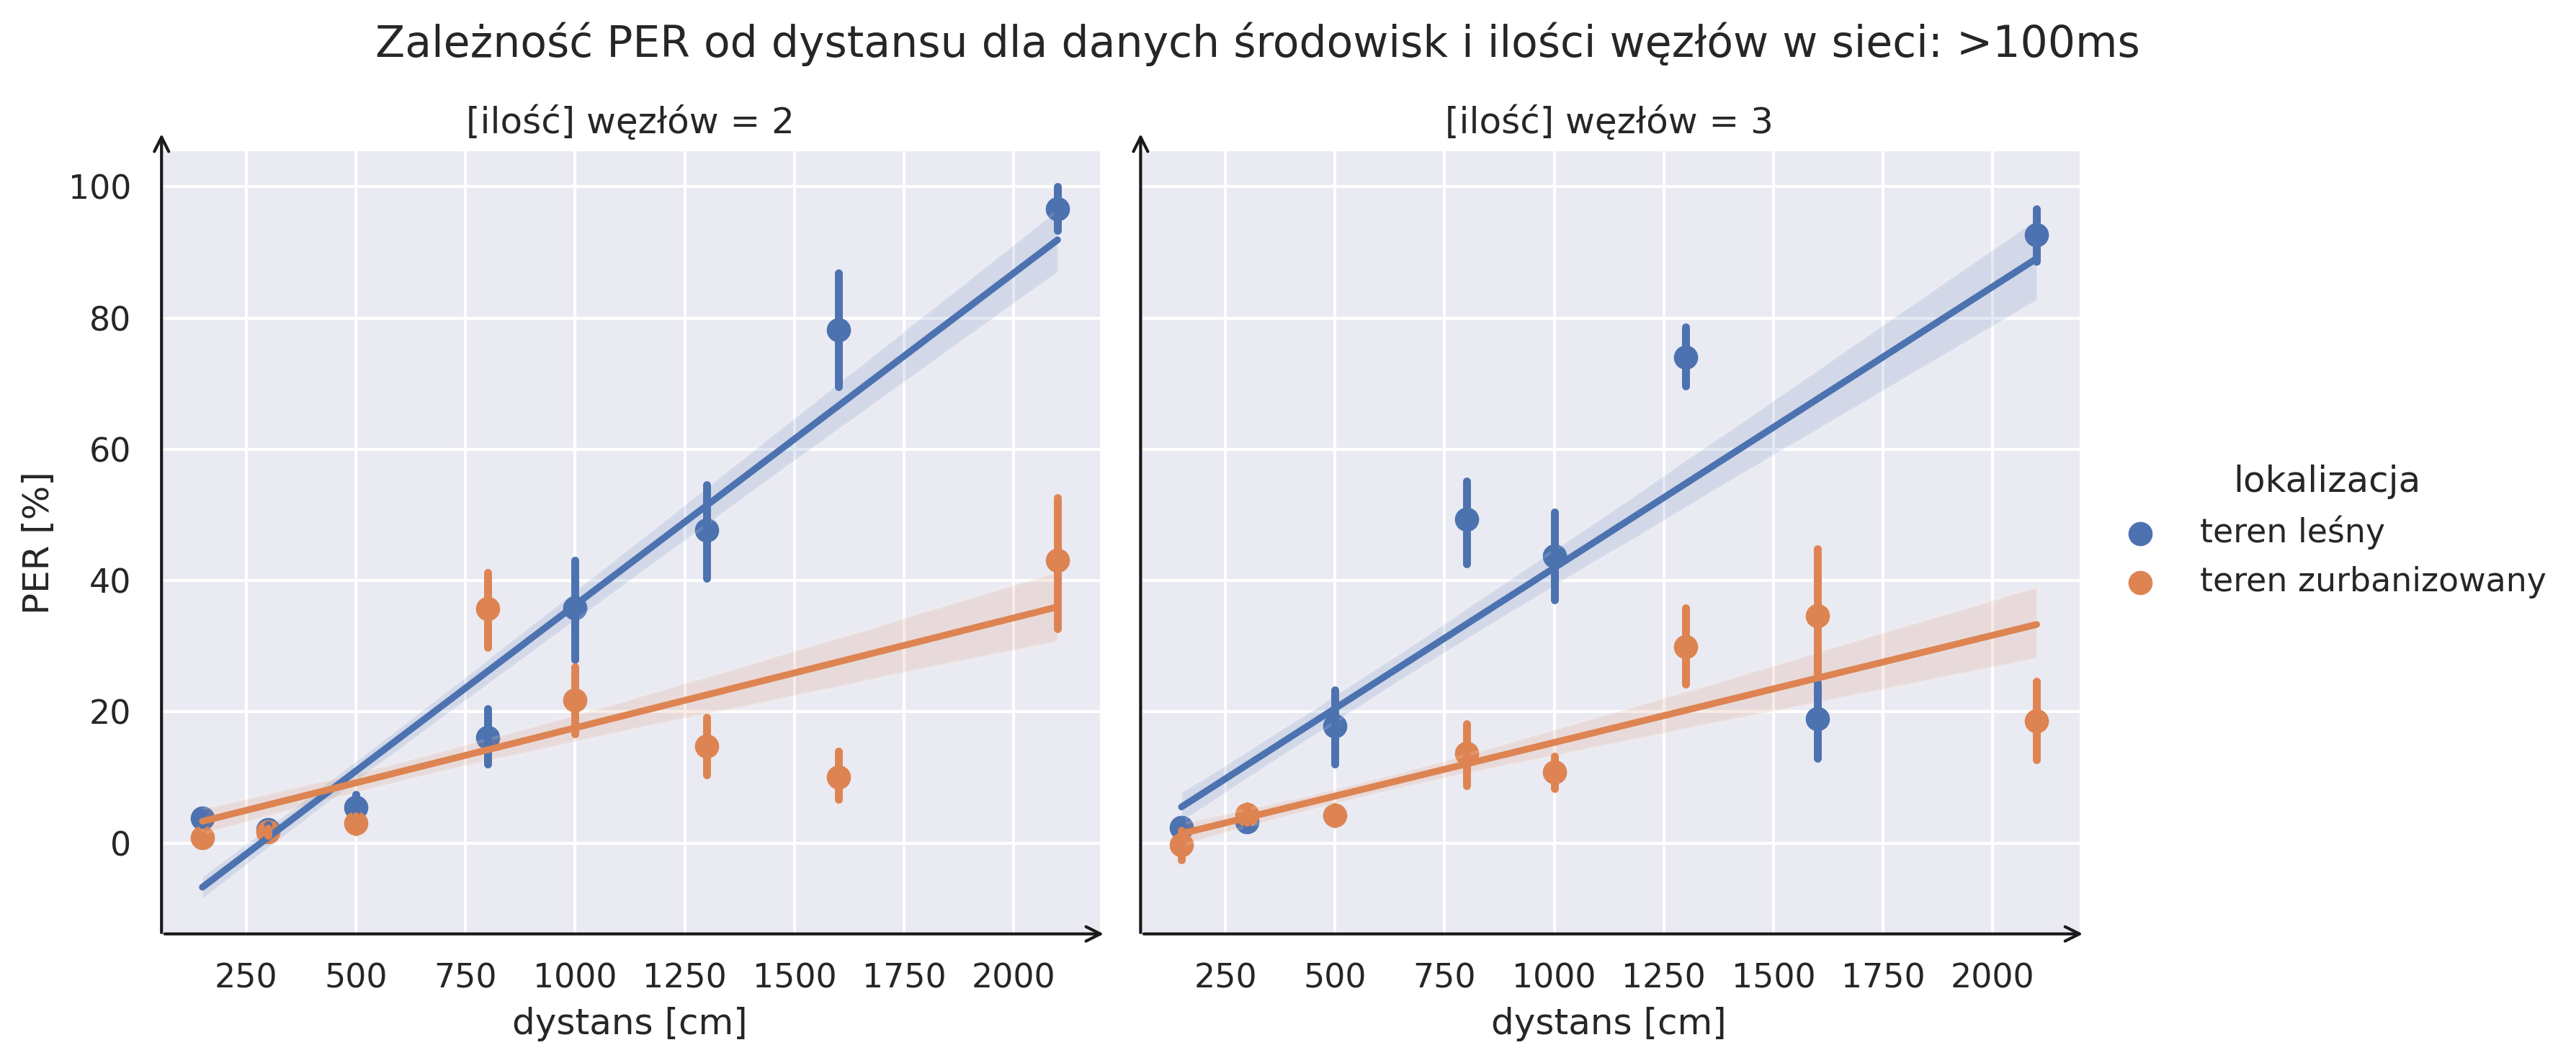
\includegraphics[width=0.99\linewidth]{per_to_distance_over_100ms_different_envs_and_nodes.png}
	\caption{Zależność \gls{PER} od dystansu dla zapytań o częstości >100ms w wybranych środowiskach i liczbę badanych węzłów}
	\label{rys:per_to_distance_over_100ms_different_envs_and_nodes}
\end{figure}

